% =====================================================================
%  CSE 402 -- Numerical Analysis Assignment
%  Topic 3: Gradient Methods
%  Roll: 2105032
%  Build:  pdflatex 2105032 ; bibtex 2105032 ; pdflatex 2105032 ; pdflatex 2105032
% =====================================================================
\documentclass[aspectratio=169, 11pt]{beamer}
% =====================================================================
%  paper-navy-beamer :: preamble.tex
%  A light "paper" Beamer theme built on Metropolis (pdfLaTeX, no shell-escape).
%
%  Visual system:
%    * light paper content slides; dark navy only for the title slide and
%      big-statement slides (projector friendly);
%    * three colours with fixed jobs: navy = structure, orange = attention,
%      teal = answers / key results (all >= 4.5:1 on the paper background);
%    * white frame header: title left, current section right, orange rule
%      underneath that doubles as a progress bar;
%    * numbered section dividers with an optional "you are here" stop strip;
%    * left-accent boxes; optional navy edge strip for problem/exercise frames.
%
%  Deck-level settings (redefine with \renewcommand after % =====================================================================
%  paper-navy-beamer :: preamble.tex
%  A light "paper" Beamer theme built on Metropolis (pdfLaTeX, no shell-escape).
%
%  Visual system:
%    * light paper content slides; dark navy only for the title slide and
%      big-statement slides (projector friendly);
%    * three colours with fixed jobs: navy = structure, orange = attention,
%      teal = answers / key results (all >= 4.5:1 on the paper background);
%    * white frame header: title left, current section right, orange rule
%      underneath that doubles as a progress bar;
%    * numbered section dividers with an optional "you are here" stop strip;
%    * left-accent boxes; optional navy edge strip for problem/exercise frames.
%
%  Deck-level settings (redefine with \renewcommand after % =====================================================================
%  paper-navy-beamer :: preamble.tex
%  A light "paper" Beamer theme built on Metropolis (pdfLaTeX, no shell-escape).
%
%  Visual system:
%    * light paper content slides; dark navy only for the title slide and
%      big-statement slides (projector friendly);
%    * three colours with fixed jobs: navy = structure, orange = attention,
%      teal = answers / key results (all >= 4.5:1 on the paper background);
%    * white frame header: title left, current section right, orange rule
%      underneath that doubles as a progress bar;
%    * numbered section dividers with an optional "you are here" stop strip;
%    * left-accent boxes; optional navy edge strip for problem/exercise frames.
%
%  Deck-level settings (redefine with \renewcommand after \input{preamble}):
%    \deckfooter   footer text                (default: short title | short author)
%    \deckkicker   small caps line above the title on the title slide (default empty)
%    \deckmeta     line under the author on the title slide (default: date)
%    \deckart      basename of the title-slide artwork PDF (default fig_title_bg)
%    \deckstops    comma list of roadmap stop labels for the section strip (default empty = no strip)
%    \stripprefix  word on the problem edge strip (default PROBLEM)
%  Per-section overrides (place right before \section):
%    \nextsectionstop{n}   which stop to highlight (0 = hide strip, > #stops = "all done")
%    \nextsectionlabel{B}  text of the big number (default: two-digit section number)
% =====================================================================

% ---------- theme ----------
\usetheme[progressbar=none, numbering=fraction, block=fill]{metropolis}
\setbeamersize{text margin left=0.9cm, text margin right=0.9cm}

% ---------- encoding / fonts ----------
\usepackage[T1]{fontenc}
\usepackage[utf8]{inputenc}
\usepackage[sfdefault, lining, scaled=0.92]{FiraSans}   % text
\usepackage[scaled=0.86]{FiraMono}                       % code
\renewcommand*\familydefault{\sfdefault}

% ---------- mathematics ----------
\usepackage{amsmath, amsthm, mathtools}
\usefonttheme{professionalfonts}       % let newtxsf set the maths fonts
\usepackage{newtxsf}                   % sans-serif maths matching Fira (load after amsmath; no amssymb, no bm)
\usepackage{nicefrac}

% ---------- graphics / tables ----------
\usepackage{graphicx}
\graphicspath{{figures/generated/}{figures/tikz/}{figures/}}
\usepackage{booktabs, array, multirow, makecell}
\usepackage{tikz}
\usetikzlibrary{arrows.meta, calc, positioning, shapes.geometric, shadows, fadings,
                decorations.pathmorphing, decorations.pathreplacing, patterns, backgrounds}
\usepackage{xcolor}
\usepackage{etoolbox}

% ---------- boxes / code / links ----------
\usepackage[most]{tcolorbox}
\usepackage{listings}
\usepackage{appendixnumberbeamer}
\usepackage{hyperref}

% =====================================================================
%  Colours
% =====================================================================
\definecolor{mNavy}{HTML}{1E3A5F}       % structure: headers, theorems   (10.9:1)
\definecolor{mOrange}{HTML}{C2410C}     % attention: alerts, problems    (5.0:1)
\definecolor{mTeal}{HTML}{0F766E}       % answers, key results           (5.3:1)
\definecolor{mRed}{HTML}{B91C1C}        % warnings / failure             (6.3:1)
\definecolor{mBlue}{HTML}{1D4ED8}       % secondary series colour         (6.5:1)
\definecolor{mGrey}{HTML}{4B5563}       % secondary text                  (7.4:1)
\definecolor{mInk}{HTML}{111827}        % body text
\definecolor{mPaper}{HTML}{FBFAF7}      % warm off-white slide background
\definecolor{mLight}{HTML}{F3F1EC}      % code background
\definecolor{mOrangeLt}{HTML}{FDBA74}   % accent text on the dark navy slides
\definecolor{mSky}{HTML}{BFDBFE}        % secondary text on the dark navy slides
\colorlet{mDarkTeal}{mNavy}             % aliases so older snippets keep working
\colorlet{mGreen}{mTeal}

\setbeamercolor{normal text}{fg=mInk, bg=mPaper}
\setbeamercolor{background canvas}{bg=mPaper}
\setbeamercolor{alerted text}{fg=mOrange}
\setbeamercolor{example text}{fg=mTeal}
\setbeamercolor{frametitle}{fg=mNavy, bg=mPaper}
\setbeamercolor{palette primary}{fg=white, bg=mNavy}     % standout (statement) slides
\setbeamercolor{footline}{fg=mGrey}
\setbeamercolor{page number in head/foot}{fg=mGrey}
\setbeamercolor{itemize item}{fg=mOrange}
\setbeamercolor{itemize subitem}{fg=mOrange}
\setbeamercolor{enumerate item}{fg=mNavy}
\setbeamercolor{section title}{fg=mNavy}

\setbeamerfont{frametitle}{size=\large, series=\bfseries}
\setbeamerfont{section title}{size=\LARGE, series=\bfseries}
\setbeamerfont{standout}{size=\LARGE, series=\bfseries}

% =====================================================================
%  Deck-level settings (defaults)
% =====================================================================
\newcommand{\deckfooter}{\insertshorttitle\quad|\quad\insertshortauthor}
\newcommand{\deckkicker}{}
\newcommand{\deckmeta}{\insertdate}
\newcommand{\deckart}{fig_title_bg}
\newcommand{\deckstops}{}
\newcommand{\stripprefix}{PROBLEM}
\setbeamertemplate{frame footer}{\deckfooter}

\makeatletter
% =====================================================================
%  Frame header: title left, current section right, progress rule below.
% =====================================================================
\newlength{\gm@track}
\newlength{\gm@prog}
\newcommand{\gm@progressrule}{%
  \setlength{\gm@track}{\textwidth}%
  \pgfmathsetlength{\gm@prog}{min(1,\insertframenumber/max(1,\inserttotalframenumber))*\gm@track}%
  {\color{mOrange}\rule{\gm@prog}{1.4pt}}{\color{mNavy!12}\rule{\dimexpr\gm@track-\gm@prog\relax}{1.4pt}}}
\setbeamertemplate{frametitle}{%
  \nointerlineskip
  \vskip 5pt
  \sbox0{\usebeamerfont{frametitle}\usebeamercolor[fg]{frametitle}\insertframetitle}%
  \sbox1{\scriptsize\bfseries\color{mOrange}\insertsectionhead}%
  \hbox to \textwidth{%
    \ifdim\dimexpr\wd0+\wd1+1.0cm\relax<\textwidth
      \box0\hfill\raise1.5pt\box1%
    \else
      \parbox[b]{\textwidth}{\raggedright
        \usebeamerfont{frametitle}\usebeamercolor[fg]{frametitle}\insertframetitle}%
    \fi}%
  \vskip 3pt
  \hbox to \textwidth{\gm@progressrule\hfil}%
}

% =====================================================================
%  Title slide: full-bleed navy, faded artwork on the right, author block.
% =====================================================================
\setbeamertemplate{title page}{%
  \begin{tikzpicture}[remember picture, overlay]
    \fill[mNavy] (current page.south west) rectangle (current page.north east);
    % \IfFileExists ignores \graphicspath, so look in the usual figure folders explicitly
    \gdef\gm@artfile{}%
    \IfFileExists{\deckart.pdf}{\xdef\gm@artfile{\deckart}}{%
      \IfFileExists{figures/generated/\deckart.pdf}{\xdef\gm@artfile{figures/generated/\deckart}}{%
        \IfFileExists{figures/\deckart.pdf}{\xdef\gm@artfile{figures/\deckart}}{}}}%
    \ifx\gm@artfile\empty\else
      \node[anchor=east, inner sep=0pt, opacity=0.9] at ([xshift=0.4cm]current page.east)
        {\includegraphics[height=1.05\paperheight]{\gm@artfile}};
      \fill[mNavy, path fading=east] (current page.south west) rectangle ([xshift=-3.4cm]current page.north east);
    \fi
    \node[anchor=north west, text width=0.62\paperwidth, align=left, inner sep=0pt]
      at ([xshift=1.0cm, yshift=-1.55cm]current page.north west) {%
        \ifx\deckkicker\empty\else{\color{mOrangeLt}\scriptsize\bfseries\deckkicker}\\[10pt]\fi
        {\color{white}\fontsize{28}{30}\selectfont\bfseries \inserttitle}\\[8pt]
        \ifx\beamer@subtitle\@empty\else{\color{mSky}\normalsize \insertsubtitle}\\[12pt]\fi
        {\color{mOrangeLt}\rule{2.2cm}{2pt}}\\[14pt]
        {\color{white}\large\bfseries \insertauthor}\\[3pt]
        {\color{mSky}\small \deckmeta}};
  \end{tikzpicture}}

% =====================================================================
%  Section dividers: big number, title, optional stop strip.
% =====================================================================
\let\gm@nextstop\relax
\let\gm@nextlabel\relax
\newcommand{\nextsectionstop}[1]{\gdef\gm@nextstop{#1}}
\newcommand{\nextsectionlabel}[1]{\gdef\gm@nextlabel{#1}}
\newcommand{\gm@secnum}{%
  \ifx\gm@nextlabel\relax\ifnum\value{section}<10 0\fi\arabic{section}\else\gm@nextlabel\fi}
\newcommand{\gm@stopstrip}{%
  \ifx\deckstops\empty\else
    \def\gm@n{0}%
    \foreach \gm@lab in \deckstops {\xdef\gm@n{\the\numexpr\gm@n+1\relax}}%
    \ifx\gm@nextstop\relax\edef\gm@cur{\arabic{section}}\else\edef\gm@cur{\gm@nextstop}\fi
    \ifnum\gm@cur>0
      \pgfmathsetmacro\gm@dx{9.6/max(1,\gm@n-1)}%
      \begin{tikzpicture}[x=\gm@dx cm]
        \draw[mNavy!25, line width=1.2pt] (1,0) -- (\gm@n,0);
        \foreach \gm@lab [count=\i] in \deckstops {%
          \ifnum\gm@cur>\gm@n
            \fill[mNavy] (\i,0) circle (2.6pt);
          \else\ifnum\i<\gm@cur
            \fill[mNavy] (\i,0) circle (2.6pt);
          \else\ifnum\i=\gm@cur
            \fill[mOrange] (\i,0) circle (4.6pt); \fill[mPaper] (\i,0) circle (1.6pt);
            \node[below=5pt, font=\scriptsize\bfseries, mOrange] at (\i,0) {\gm@lab};
          \else
            \fill[mPaper] (\i,0) circle (2.6pt); \draw[mNavy!45, line width=0.8pt] (\i,0) circle (2.6pt);
          \fi\fi\fi}
        \ifnum\gm@cur>\gm@n \node[below=5pt, font=\scriptsize\bfseries, mOrange] at ({(1+\gm@n)/2},0) {recap}; \fi
      \end{tikzpicture}%
    \fi
  \fi}
\setbeamertemplate{section page}{%
  \begin{minipage}{0.86\textwidth}
    \raggedright
    {\fontsize{46}{46}\selectfont\bfseries\color{mOrange}\gm@secnum}\\[4pt]
    {\usebeamerfont{section title}\usebeamercolor[fg]{section title}\insertsectionhead}\\[2pt]
    {\color{mOrange}\rule{1.6cm}{2pt}}\\[18pt]
    \gm@stopstrip
  \end{minipage}%
  \global\let\gm@nextstop\relax
  \global\let\gm@nextlabel\relax}

% =====================================================================
%  Tighter display maths and lists (Fira Sans is taller than CM).
% =====================================================================
\newcommand{\gm@tightdisplay}{%
  \setlength{\abovedisplayskip}{5pt plus 2pt minus 2pt}%
  \setlength{\belowdisplayskip}{5pt plus 2pt minus 2pt}%
  \setlength{\abovedisplayshortskip}{2pt plus 2pt}%
  \setlength{\belowdisplayshortskip}{4pt plus 2pt minus 2pt}}
\appto\normalsize{\gm@tightdisplay}
\appto\small{\gm@tightdisplay}
\appto\footnotesize{\gm@tightdisplay}
\setbeamertemplate{itemize/enumerate body begin}{\setlength{\itemsep}{1pt}}
\setbeamertemplate{itemize/enumerate subbody begin}{\setlength{\itemsep}{0pt}}
\setlength{\leftmargini}{1.2em}

% =====================================================================
%  Problem / exercise frames: navy edge strip with an id, step dots.
% =====================================================================
\gdef\gmprob{}
\newcommand{\setprob}[1]{\gdef\gmprob{#1}}
\setbeamertemplate{background}{%
  \ifx\gmprob\empty\else
  \begin{tikzpicture}
    \useasboundingbox (0,0) rectangle (\paperwidth,\paperheight);
    \fill[mNavy] (0,0.8cm) rectangle (0.36cm,\paperheight);   % stops above the footer
    \node[rotate=90, text=white, font=\scriptsize\bfseries, inner sep=0pt] at (0.18cm,0.55\paperheight)
      {\stripprefix\ \gmprob};
  \end{tikzpicture}%
  \fi}
\def\gm@dots#1#2#3{%
  \ifnum#1>#3\relax\else
    \ifnum#1>#2\relax{\color{mNavy!25}\textbullet}\else{\color{mOrange}\textbullet}\fi
    \expandafter\gm@dots\expandafter{\the\numexpr#1+1\relax}{#2}{#3}%
  \fi}
\newcommand{\stepdots}[2]{{\normalsize\gm@dots{1}{#1}{#2}}}
\makeatother

% \probtitle{M1}{Stationary points}  -> "Problem M1 · Stationary points"
% \soltitle{M1}{2}{4}                 -> "Problem M1 · Solution 2/4 ••○○"
\newcommand{\probtitle}[2]{Problem #1 \textperiodcentered\ #2}
\newcommand{\soltitle}[3]{Problem #1 \textperiodcentered\ Solution #2/#3 \;\stepdots{#2}{#3}}

% =====================================================================
%  Boxes: coloured bar on the left, tinted background, coloured title.
% =====================================================================
\tcbset{
  gmbase/.style={enhanced, breakable=false, frame hidden, sharp corners,
                 borderline west={2.6pt}{0pt}{#1},
                 colback=#1!6!mPaper, colbacktitle=#1!6!mPaper, coltitle=#1,
                 titlerule=0pt, toptitle=3pt, bottomtitle=-1pt,
                 left=8pt, right=6pt, top=3pt, bottom=4pt,
                 fonttitle=\bfseries\small, fontupper=\small,
                 before skip=5pt, after skip=5pt}
}
\newtcolorbox{probbox}[1][]{gmbase=mOrange, title={#1}}   % problem statements, tasks
\newtcolorbox{thmbox}[1][]{gmbase=mNavy, title={#1}}      % theorems, definitions, algorithms
\newtcolorbox{keybox}[1][]{gmbase=mTeal, title={#1}}      % key ideas, insights, takeaways
\newtcolorbox{warnbox}[1][]{gmbase=mRed, title={#1}}      % caveats, pitfalls

% boxed answers (works in text and in maths): rounded teal outline
\newtcbox{\anstcb}{on line, enhanced, colback=mTeal!8!mPaper, colframe=mTeal, boxrule=0.7pt,
  arc=2.5pt, left=2.5pt, right=2.5pt, top=1pt, bottom=1pt, boxsep=0.6pt}
\newcommand{\ans}[1]{\text{\anstcb{$\displaystyle #1$}}}

% =====================================================================
%  Statement slides: dark navy, one big idea in large type.
%  \statement{KICKER}{Big sentence (\\ allowed)}{small follow-up}
% =====================================================================
\newcommand{\statement}[3]{%
  \begin{frame}[standout]
    \begin{minipage}{0.84\textwidth}\centering
      {\color{mOrangeLt}\scriptsize\bfseries #1\par}\vspace{10pt}
      {\LARGE\bfseries\color{white} #2\par}\vspace{12pt}
      {\color{mOrangeLt}\rule{1.6cm}{1.6pt}\par}\vspace{10pt}
      {\color{mSky}\normalsize\mdseries #3\par}
    \end{minipage}
  \end{frame}}

% =====================================================================
%  Small generic maths helpers
% =====================================================================
\providecommand{\R}{\mathbb{R}}
\providecommand{\E}{\mathbb{E}}
\providecommand{\T}{^{\mathsf T}}
\providecommand{\norm}[1]{\left\lVert #1 \right\rVert}
\providecommand{\abs}[1]{\left\lvert #1 \right\rvert}
\DeclareMathOperator*{\argmin}{arg\,min}
\DeclareMathOperator*{\argmax}{arg\,max}
\DeclareMathOperator{\diag}{diag}

% =====================================================================
%  Code listings
% =====================================================================
\lstdefinestyle{py}{
  language=Python, basicstyle=\ttfamily\scriptsize,
  keywordstyle=\color{mBlue}\bfseries, commentstyle=\color{mGrey}\itshape,
  stringstyle=\color{mTeal}, showstringspaces=false,
  frame=leftline, framerule=2.6pt, rulecolor=\color{mNavy}, backgroundcolor=\color{mLight},
  xleftmargin=6pt, xrightmargin=2pt, framesep=5pt, columns=fullflexible, keepspaces=true}

% =====================================================================
%  Bibliography: numbered labels, compact entries
% =====================================================================
\setbeamertemplate{bibliography item}{\insertbiblabel}
\setbeamertemplate{bibliography entry title}{}
\setbeamertemplate{bibliography entry location}{}
\setbeamertemplate{bibliography entry note}{}
):
%    \deckfooter   footer text                (default: short title | short author)
%    \deckkicker   small caps line above the title on the title slide (default empty)
%    \deckmeta     line under the author on the title slide (default: date)
%    \deckart      basename of the title-slide artwork PDF (default fig_title_bg)
%    \deckstops    comma list of roadmap stop labels for the section strip (default empty = no strip)
%    \stripprefix  word on the problem edge strip (default PROBLEM)
%  Per-section overrides (place right before \section):
%    \nextsectionstop{n}   which stop to highlight (0 = hide strip, > #stops = "all done")
%    \nextsectionlabel{B}  text of the big number (default: two-digit section number)
% =====================================================================

% ---------- theme ----------
\usetheme[progressbar=none, numbering=fraction, block=fill]{metropolis}
\setbeamersize{text margin left=0.9cm, text margin right=0.9cm}

% ---------- encoding / fonts ----------
\usepackage[T1]{fontenc}
\usepackage[utf8]{inputenc}
\usepackage[sfdefault, lining, scaled=0.92]{FiraSans}   % text
\usepackage[scaled=0.86]{FiraMono}                       % code
\renewcommand*\familydefault{\sfdefault}

% ---------- mathematics ----------
\usepackage{amsmath, amsthm, mathtools}
\usefonttheme{professionalfonts}       % let newtxsf set the maths fonts
\usepackage{newtxsf}                   % sans-serif maths matching Fira (load after amsmath; no amssymb, no bm)
\usepackage{nicefrac}

% ---------- graphics / tables ----------
\usepackage{graphicx}
\graphicspath{{figures/generated/}{figures/tikz/}{figures/}}
\usepackage{booktabs, array, multirow, makecell}
\usepackage{tikz}
\usetikzlibrary{arrows.meta, calc, positioning, shapes.geometric, shadows, fadings,
                decorations.pathmorphing, decorations.pathreplacing, patterns, backgrounds}
\usepackage{xcolor}
\usepackage{etoolbox}

% ---------- boxes / code / links ----------
\usepackage[most]{tcolorbox}
\usepackage{listings}
\usepackage{appendixnumberbeamer}
\usepackage{hyperref}

% =====================================================================
%  Colours
% =====================================================================
\definecolor{mNavy}{HTML}{1E3A5F}       % structure: headers, theorems   (10.9:1)
\definecolor{mOrange}{HTML}{C2410C}     % attention: alerts, problems    (5.0:1)
\definecolor{mTeal}{HTML}{0F766E}       % answers, key results           (5.3:1)
\definecolor{mRed}{HTML}{B91C1C}        % warnings / failure             (6.3:1)
\definecolor{mBlue}{HTML}{1D4ED8}       % secondary series colour         (6.5:1)
\definecolor{mGrey}{HTML}{4B5563}       % secondary text                  (7.4:1)
\definecolor{mInk}{HTML}{111827}        % body text
\definecolor{mPaper}{HTML}{FBFAF7}      % warm off-white slide background
\definecolor{mLight}{HTML}{F3F1EC}      % code background
\definecolor{mOrangeLt}{HTML}{FDBA74}   % accent text on the dark navy slides
\definecolor{mSky}{HTML}{BFDBFE}        % secondary text on the dark navy slides
\colorlet{mDarkTeal}{mNavy}             % aliases so older snippets keep working
\colorlet{mGreen}{mTeal}

\setbeamercolor{normal text}{fg=mInk, bg=mPaper}
\setbeamercolor{background canvas}{bg=mPaper}
\setbeamercolor{alerted text}{fg=mOrange}
\setbeamercolor{example text}{fg=mTeal}
\setbeamercolor{frametitle}{fg=mNavy, bg=mPaper}
\setbeamercolor{palette primary}{fg=white, bg=mNavy}     % standout (statement) slides
\setbeamercolor{footline}{fg=mGrey}
\setbeamercolor{page number in head/foot}{fg=mGrey}
\setbeamercolor{itemize item}{fg=mOrange}
\setbeamercolor{itemize subitem}{fg=mOrange}
\setbeamercolor{enumerate item}{fg=mNavy}
\setbeamercolor{section title}{fg=mNavy}

\setbeamerfont{frametitle}{size=\large, series=\bfseries}
\setbeamerfont{section title}{size=\LARGE, series=\bfseries}
\setbeamerfont{standout}{size=\LARGE, series=\bfseries}

% =====================================================================
%  Deck-level settings (defaults)
% =====================================================================
\newcommand{\deckfooter}{\insertshorttitle\quad|\quad\insertshortauthor}
\newcommand{\deckkicker}{}
\newcommand{\deckmeta}{\insertdate}
\newcommand{\deckart}{fig_title_bg}
\newcommand{\deckstops}{}
\newcommand{\stripprefix}{PROBLEM}
\setbeamertemplate{frame footer}{\deckfooter}

\makeatletter
% =====================================================================
%  Frame header: title left, current section right, progress rule below.
% =====================================================================
\newlength{\gm@track}
\newlength{\gm@prog}
\newcommand{\gm@progressrule}{%
  \setlength{\gm@track}{\textwidth}%
  \pgfmathsetlength{\gm@prog}{min(1,\insertframenumber/max(1,\inserttotalframenumber))*\gm@track}%
  {\color{mOrange}\rule{\gm@prog}{1.4pt}}{\color{mNavy!12}\rule{\dimexpr\gm@track-\gm@prog\relax}{1.4pt}}}
\setbeamertemplate{frametitle}{%
  \nointerlineskip
  \vskip 5pt
  \sbox0{\usebeamerfont{frametitle}\usebeamercolor[fg]{frametitle}\insertframetitle}%
  \sbox1{\scriptsize\bfseries\color{mOrange}\insertsectionhead}%
  \hbox to \textwidth{%
    \ifdim\dimexpr\wd0+\wd1+1.0cm\relax<\textwidth
      \box0\hfill\raise1.5pt\box1%
    \else
      \parbox[b]{\textwidth}{\raggedright
        \usebeamerfont{frametitle}\usebeamercolor[fg]{frametitle}\insertframetitle}%
    \fi}%
  \vskip 3pt
  \hbox to \textwidth{\gm@progressrule\hfil}%
}

% =====================================================================
%  Title slide: full-bleed navy, faded artwork on the right, author block.
% =====================================================================
\setbeamertemplate{title page}{%
  \begin{tikzpicture}[remember picture, overlay]
    \fill[mNavy] (current page.south west) rectangle (current page.north east);
    % \IfFileExists ignores \graphicspath, so look in the usual figure folders explicitly
    \gdef\gm@artfile{}%
    \IfFileExists{\deckart.pdf}{\xdef\gm@artfile{\deckart}}{%
      \IfFileExists{figures/generated/\deckart.pdf}{\xdef\gm@artfile{figures/generated/\deckart}}{%
        \IfFileExists{figures/\deckart.pdf}{\xdef\gm@artfile{figures/\deckart}}{}}}%
    \ifx\gm@artfile\empty\else
      \node[anchor=east, inner sep=0pt, opacity=0.9] at ([xshift=0.4cm]current page.east)
        {\includegraphics[height=1.05\paperheight]{\gm@artfile}};
      \fill[mNavy, path fading=east] (current page.south west) rectangle ([xshift=-3.4cm]current page.north east);
    \fi
    \node[anchor=north west, text width=0.62\paperwidth, align=left, inner sep=0pt]
      at ([xshift=1.0cm, yshift=-1.55cm]current page.north west) {%
        \ifx\deckkicker\empty\else{\color{mOrangeLt}\scriptsize\bfseries\deckkicker}\\[10pt]\fi
        {\color{white}\fontsize{28}{30}\selectfont\bfseries \inserttitle}\\[8pt]
        \ifx\beamer@subtitle\@empty\else{\color{mSky}\normalsize \insertsubtitle}\\[12pt]\fi
        {\color{mOrangeLt}\rule{2.2cm}{2pt}}\\[14pt]
        {\color{white}\large\bfseries \insertauthor}\\[3pt]
        {\color{mSky}\small \deckmeta}};
  \end{tikzpicture}}

% =====================================================================
%  Section dividers: big number, title, optional stop strip.
% =====================================================================
\let\gm@nextstop\relax
\let\gm@nextlabel\relax
\newcommand{\nextsectionstop}[1]{\gdef\gm@nextstop{#1}}
\newcommand{\nextsectionlabel}[1]{\gdef\gm@nextlabel{#1}}
\newcommand{\gm@secnum}{%
  \ifx\gm@nextlabel\relax\ifnum\value{section}<10 0\fi\arabic{section}\else\gm@nextlabel\fi}
\newcommand{\gm@stopstrip}{%
  \ifx\deckstops\empty\else
    \def\gm@n{0}%
    \foreach \gm@lab in \deckstops {\xdef\gm@n{\the\numexpr\gm@n+1\relax}}%
    \ifx\gm@nextstop\relax\edef\gm@cur{\arabic{section}}\else\edef\gm@cur{\gm@nextstop}\fi
    \ifnum\gm@cur>0
      \pgfmathsetmacro\gm@dx{9.6/max(1,\gm@n-1)}%
      \begin{tikzpicture}[x=\gm@dx cm]
        \draw[mNavy!25, line width=1.2pt] (1,0) -- (\gm@n,0);
        \foreach \gm@lab [count=\i] in \deckstops {%
          \ifnum\gm@cur>\gm@n
            \fill[mNavy] (\i,0) circle (2.6pt);
          \else\ifnum\i<\gm@cur
            \fill[mNavy] (\i,0) circle (2.6pt);
          \else\ifnum\i=\gm@cur
            \fill[mOrange] (\i,0) circle (4.6pt); \fill[mPaper] (\i,0) circle (1.6pt);
            \node[below=5pt, font=\scriptsize\bfseries, mOrange] at (\i,0) {\gm@lab};
          \else
            \fill[mPaper] (\i,0) circle (2.6pt); \draw[mNavy!45, line width=0.8pt] (\i,0) circle (2.6pt);
          \fi\fi\fi}
        \ifnum\gm@cur>\gm@n \node[below=5pt, font=\scriptsize\bfseries, mOrange] at ({(1+\gm@n)/2},0) {recap}; \fi
      \end{tikzpicture}%
    \fi
  \fi}
\setbeamertemplate{section page}{%
  \begin{minipage}{0.86\textwidth}
    \raggedright
    {\fontsize{46}{46}\selectfont\bfseries\color{mOrange}\gm@secnum}\\[4pt]
    {\usebeamerfont{section title}\usebeamercolor[fg]{section title}\insertsectionhead}\\[2pt]
    {\color{mOrange}\rule{1.6cm}{2pt}}\\[18pt]
    \gm@stopstrip
  \end{minipage}%
  \global\let\gm@nextstop\relax
  \global\let\gm@nextlabel\relax}

% =====================================================================
%  Tighter display maths and lists (Fira Sans is taller than CM).
% =====================================================================
\newcommand{\gm@tightdisplay}{%
  \setlength{\abovedisplayskip}{5pt plus 2pt minus 2pt}%
  \setlength{\belowdisplayskip}{5pt plus 2pt minus 2pt}%
  \setlength{\abovedisplayshortskip}{2pt plus 2pt}%
  \setlength{\belowdisplayshortskip}{4pt plus 2pt minus 2pt}}
\appto\normalsize{\gm@tightdisplay}
\appto\small{\gm@tightdisplay}
\appto\footnotesize{\gm@tightdisplay}
\setbeamertemplate{itemize/enumerate body begin}{\setlength{\itemsep}{1pt}}
\setbeamertemplate{itemize/enumerate subbody begin}{\setlength{\itemsep}{0pt}}
\setlength{\leftmargini}{1.2em}

% =====================================================================
%  Problem / exercise frames: navy edge strip with an id, step dots.
% =====================================================================
\gdef\gmprob{}
\newcommand{\setprob}[1]{\gdef\gmprob{#1}}
\setbeamertemplate{background}{%
  \ifx\gmprob\empty\else
  \begin{tikzpicture}
    \useasboundingbox (0,0) rectangle (\paperwidth,\paperheight);
    \fill[mNavy] (0,0.8cm) rectangle (0.36cm,\paperheight);   % stops above the footer
    \node[rotate=90, text=white, font=\scriptsize\bfseries, inner sep=0pt] at (0.18cm,0.55\paperheight)
      {\stripprefix\ \gmprob};
  \end{tikzpicture}%
  \fi}
\def\gm@dots#1#2#3{%
  \ifnum#1>#3\relax\else
    \ifnum#1>#2\relax{\color{mNavy!25}\textbullet}\else{\color{mOrange}\textbullet}\fi
    \expandafter\gm@dots\expandafter{\the\numexpr#1+1\relax}{#2}{#3}%
  \fi}
\newcommand{\stepdots}[2]{{\normalsize\gm@dots{1}{#1}{#2}}}
\makeatother

% \probtitle{M1}{Stationary points}  -> "Problem M1 · Stationary points"
% \soltitle{M1}{2}{4}                 -> "Problem M1 · Solution 2/4 ••○○"
\newcommand{\probtitle}[2]{Problem #1 \textperiodcentered\ #2}
\newcommand{\soltitle}[3]{Problem #1 \textperiodcentered\ Solution #2/#3 \;\stepdots{#2}{#3}}

% =====================================================================
%  Boxes: coloured bar on the left, tinted background, coloured title.
% =====================================================================
\tcbset{
  gmbase/.style={enhanced, breakable=false, frame hidden, sharp corners,
                 borderline west={2.6pt}{0pt}{#1},
                 colback=#1!6!mPaper, colbacktitle=#1!6!mPaper, coltitle=#1,
                 titlerule=0pt, toptitle=3pt, bottomtitle=-1pt,
                 left=8pt, right=6pt, top=3pt, bottom=4pt,
                 fonttitle=\bfseries\small, fontupper=\small,
                 before skip=5pt, after skip=5pt}
}
\newtcolorbox{probbox}[1][]{gmbase=mOrange, title={#1}}   % problem statements, tasks
\newtcolorbox{thmbox}[1][]{gmbase=mNavy, title={#1}}      % theorems, definitions, algorithms
\newtcolorbox{keybox}[1][]{gmbase=mTeal, title={#1}}      % key ideas, insights, takeaways
\newtcolorbox{warnbox}[1][]{gmbase=mRed, title={#1}}      % caveats, pitfalls

% boxed answers (works in text and in maths): rounded teal outline
\newtcbox{\anstcb}{on line, enhanced, colback=mTeal!8!mPaper, colframe=mTeal, boxrule=0.7pt,
  arc=2.5pt, left=2.5pt, right=2.5pt, top=1pt, bottom=1pt, boxsep=0.6pt}
\newcommand{\ans}[1]{\text{\anstcb{$\displaystyle #1$}}}

% =====================================================================
%  Statement slides: dark navy, one big idea in large type.
%  \statement{KICKER}{Big sentence (\\ allowed)}{small follow-up}
% =====================================================================
\newcommand{\statement}[3]{%
  \begin{frame}[standout]
    \begin{minipage}{0.84\textwidth}\centering
      {\color{mOrangeLt}\scriptsize\bfseries #1\par}\vspace{10pt}
      {\LARGE\bfseries\color{white} #2\par}\vspace{12pt}
      {\color{mOrangeLt}\rule{1.6cm}{1.6pt}\par}\vspace{10pt}
      {\color{mSky}\normalsize\mdseries #3\par}
    \end{minipage}
  \end{frame}}

% =====================================================================
%  Small generic maths helpers
% =====================================================================
\providecommand{\R}{\mathbb{R}}
\providecommand{\E}{\mathbb{E}}
\providecommand{\T}{^{\mathsf T}}
\providecommand{\norm}[1]{\left\lVert #1 \right\rVert}
\providecommand{\abs}[1]{\left\lvert #1 \right\rvert}
\DeclareMathOperator*{\argmin}{arg\,min}
\DeclareMathOperator*{\argmax}{arg\,max}
\DeclareMathOperator{\diag}{diag}

% =====================================================================
%  Code listings
% =====================================================================
\lstdefinestyle{py}{
  language=Python, basicstyle=\ttfamily\scriptsize,
  keywordstyle=\color{mBlue}\bfseries, commentstyle=\color{mGrey}\itshape,
  stringstyle=\color{mTeal}, showstringspaces=false,
  frame=leftline, framerule=2.6pt, rulecolor=\color{mNavy}, backgroundcolor=\color{mLight},
  xleftmargin=6pt, xrightmargin=2pt, framesep=5pt, columns=fullflexible, keepspaces=true}

% =====================================================================
%  Bibliography: numbered labels, compact entries
% =====================================================================
\setbeamertemplate{bibliography item}{\insertbiblabel}
\setbeamertemplate{bibliography entry title}{}
\setbeamertemplate{bibliography entry location}{}
\setbeamertemplate{bibliography entry note}{}
):
%    \deckfooter   footer text                (default: short title | short author)
%    \deckkicker   small caps line above the title on the title slide (default empty)
%    \deckmeta     line under the author on the title slide (default: date)
%    \deckart      basename of the title-slide artwork PDF (default fig_title_bg)
%    \deckstops    comma list of roadmap stop labels for the section strip (default empty = no strip)
%    \stripprefix  word on the problem edge strip (default PROBLEM)
%  Per-section overrides (place right before \section):
%    \nextsectionstop{n}   which stop to highlight (0 = hide strip, > #stops = "all done")
%    \nextsectionlabel{B}  text of the big number (default: two-digit section number)
% =====================================================================

% ---------- theme ----------
\usetheme[progressbar=none, numbering=fraction, block=fill]{metropolis}
\setbeamersize{text margin left=0.9cm, text margin right=0.9cm}

% ---------- encoding / fonts ----------
\usepackage[T1]{fontenc}
\usepackage[utf8]{inputenc}
\usepackage[sfdefault, lining, scaled=0.92]{FiraSans}   % text
\usepackage[scaled=0.86]{FiraMono}                       % code
\renewcommand*\familydefault{\sfdefault}

% ---------- mathematics ----------
\usepackage{amsmath, amsthm, mathtools}
\usefonttheme{professionalfonts}       % let newtxsf set the maths fonts
\usepackage{newtxsf}                   % sans-serif maths matching Fira (load after amsmath; no amssymb, no bm)
\usepackage{nicefrac}

% ---------- graphics / tables ----------
\usepackage{graphicx}
\graphicspath{{figures/generated/}{figures/tikz/}{figures/}}
\usepackage{booktabs, array, multirow, makecell}
\usepackage{tikz}
\usetikzlibrary{arrows.meta, calc, positioning, shapes.geometric, shadows, fadings,
                decorations.pathmorphing, decorations.pathreplacing, patterns, backgrounds}
\usepackage{xcolor}
\usepackage{etoolbox}

% ---------- boxes / code / links ----------
\usepackage[most]{tcolorbox}
\usepackage{listings}
\usepackage{appendixnumberbeamer}
\usepackage{hyperref}

% =====================================================================
%  Colours
% =====================================================================
\definecolor{mNavy}{HTML}{1E3A5F}       % structure: headers, theorems   (10.9:1)
\definecolor{mOrange}{HTML}{C2410C}     % attention: alerts, problems    (5.0:1)
\definecolor{mTeal}{HTML}{0F766E}       % answers, key results           (5.3:1)
\definecolor{mRed}{HTML}{B91C1C}        % warnings / failure             (6.3:1)
\definecolor{mBlue}{HTML}{1D4ED8}       % secondary series colour         (6.5:1)
\definecolor{mGrey}{HTML}{4B5563}       % secondary text                  (7.4:1)
\definecolor{mInk}{HTML}{111827}        % body text
\definecolor{mPaper}{HTML}{FBFAF7}      % warm off-white slide background
\definecolor{mLight}{HTML}{F3F1EC}      % code background
\definecolor{mOrangeLt}{HTML}{FDBA74}   % accent text on the dark navy slides
\definecolor{mSky}{HTML}{BFDBFE}        % secondary text on the dark navy slides
\colorlet{mDarkTeal}{mNavy}             % aliases so older snippets keep working
\colorlet{mGreen}{mTeal}

\setbeamercolor{normal text}{fg=mInk, bg=mPaper}
\setbeamercolor{background canvas}{bg=mPaper}
\setbeamercolor{alerted text}{fg=mOrange}
\setbeamercolor{example text}{fg=mTeal}
\setbeamercolor{frametitle}{fg=mNavy, bg=mPaper}
\setbeamercolor{palette primary}{fg=white, bg=mNavy}     % standout (statement) slides
\setbeamercolor{footline}{fg=mGrey}
\setbeamercolor{page number in head/foot}{fg=mGrey}
\setbeamercolor{itemize item}{fg=mOrange}
\setbeamercolor{itemize subitem}{fg=mOrange}
\setbeamercolor{enumerate item}{fg=mNavy}
\setbeamercolor{section title}{fg=mNavy}

\setbeamerfont{frametitle}{size=\large, series=\bfseries}
\setbeamerfont{section title}{size=\LARGE, series=\bfseries}
\setbeamerfont{standout}{size=\LARGE, series=\bfseries}

% =====================================================================
%  Deck-level settings (defaults)
% =====================================================================
\newcommand{\deckfooter}{\insertshorttitle\quad|\quad\insertshortauthor}
\newcommand{\deckkicker}{}
\newcommand{\deckmeta}{\insertdate}
\newcommand{\deckart}{fig_title_bg}
\newcommand{\deckstops}{}
\newcommand{\stripprefix}{PROBLEM}
\setbeamertemplate{frame footer}{\deckfooter}

\makeatletter
% =====================================================================
%  Frame header: title left, current section right, progress rule below.
% =====================================================================
\newlength{\gm@track}
\newlength{\gm@prog}
\newcommand{\gm@progressrule}{%
  \setlength{\gm@track}{\textwidth}%
  \pgfmathsetlength{\gm@prog}{min(1,\insertframenumber/max(1,\inserttotalframenumber))*\gm@track}%
  {\color{mOrange}\rule{\gm@prog}{1.4pt}}{\color{mNavy!12}\rule{\dimexpr\gm@track-\gm@prog\relax}{1.4pt}}}
\setbeamertemplate{frametitle}{%
  \nointerlineskip
  \vskip 5pt
  \sbox0{\usebeamerfont{frametitle}\usebeamercolor[fg]{frametitle}\insertframetitle}%
  \sbox1{\scriptsize\bfseries\color{mOrange}\insertsectionhead}%
  \hbox to \textwidth{%
    \ifdim\dimexpr\wd0+\wd1+1.0cm\relax<\textwidth
      \box0\hfill\raise1.5pt\box1%
    \else
      \parbox[b]{\textwidth}{\raggedright
        \usebeamerfont{frametitle}\usebeamercolor[fg]{frametitle}\insertframetitle}%
    \fi}%
  \vskip 3pt
  \hbox to \textwidth{\gm@progressrule\hfil}%
}

% =====================================================================
%  Title slide: full-bleed navy, faded artwork on the right, author block.
% =====================================================================
\setbeamertemplate{title page}{%
  \begin{tikzpicture}[remember picture, overlay]
    \fill[mNavy] (current page.south west) rectangle (current page.north east);
    % \IfFileExists ignores \graphicspath, so look in the usual figure folders explicitly
    \gdef\gm@artfile{}%
    \IfFileExists{\deckart.pdf}{\xdef\gm@artfile{\deckart}}{%
      \IfFileExists{figures/generated/\deckart.pdf}{\xdef\gm@artfile{figures/generated/\deckart}}{%
        \IfFileExists{figures/\deckart.pdf}{\xdef\gm@artfile{figures/\deckart}}{}}}%
    \ifx\gm@artfile\empty\else
      \node[anchor=east, inner sep=0pt, opacity=0.9] at ([xshift=0.4cm]current page.east)
        {\includegraphics[height=1.05\paperheight]{\gm@artfile}};
      \fill[mNavy, path fading=east] (current page.south west) rectangle ([xshift=-3.4cm]current page.north east);
    \fi
    \node[anchor=north west, text width=0.62\paperwidth, align=left, inner sep=0pt]
      at ([xshift=1.0cm, yshift=-1.55cm]current page.north west) {%
        \ifx\deckkicker\empty\else{\color{mOrangeLt}\scriptsize\bfseries\deckkicker}\\[10pt]\fi
        {\color{white}\fontsize{28}{30}\selectfont\bfseries \inserttitle}\\[8pt]
        \ifx\beamer@subtitle\@empty\else{\color{mSky}\normalsize \insertsubtitle}\\[12pt]\fi
        {\color{mOrangeLt}\rule{2.2cm}{2pt}}\\[14pt]
        {\color{white}\large\bfseries \insertauthor}\\[3pt]
        {\color{mSky}\small \deckmeta}};
  \end{tikzpicture}}

% =====================================================================
%  Section dividers: big number, title, optional stop strip.
% =====================================================================
\let\gm@nextstop\relax
\let\gm@nextlabel\relax
\newcommand{\nextsectionstop}[1]{\gdef\gm@nextstop{#1}}
\newcommand{\nextsectionlabel}[1]{\gdef\gm@nextlabel{#1}}
\newcommand{\gm@secnum}{%
  \ifx\gm@nextlabel\relax\ifnum\value{section}<10 0\fi\arabic{section}\else\gm@nextlabel\fi}
\newcommand{\gm@stopstrip}{%
  \ifx\deckstops\empty\else
    \def\gm@n{0}%
    \foreach \gm@lab in \deckstops {\xdef\gm@n{\the\numexpr\gm@n+1\relax}}%
    \ifx\gm@nextstop\relax\edef\gm@cur{\arabic{section}}\else\edef\gm@cur{\gm@nextstop}\fi
    \ifnum\gm@cur>0
      \pgfmathsetmacro\gm@dx{9.6/max(1,\gm@n-1)}%
      \begin{tikzpicture}[x=\gm@dx cm]
        \draw[mNavy!25, line width=1.2pt] (1,0) -- (\gm@n,0);
        \foreach \gm@lab [count=\i] in \deckstops {%
          \ifnum\gm@cur>\gm@n
            \fill[mNavy] (\i,0) circle (2.6pt);
          \else\ifnum\i<\gm@cur
            \fill[mNavy] (\i,0) circle (2.6pt);
          \else\ifnum\i=\gm@cur
            \fill[mOrange] (\i,0) circle (4.6pt); \fill[mPaper] (\i,0) circle (1.6pt);
            \node[below=5pt, font=\scriptsize\bfseries, mOrange] at (\i,0) {\gm@lab};
          \else
            \fill[mPaper] (\i,0) circle (2.6pt); \draw[mNavy!45, line width=0.8pt] (\i,0) circle (2.6pt);
          \fi\fi\fi}
        \ifnum\gm@cur>\gm@n \node[below=5pt, font=\scriptsize\bfseries, mOrange] at ({(1+\gm@n)/2},0) {recap}; \fi
      \end{tikzpicture}%
    \fi
  \fi}
\setbeamertemplate{section page}{%
  \begin{minipage}{0.86\textwidth}
    \raggedright
    {\fontsize{46}{46}\selectfont\bfseries\color{mOrange}\gm@secnum}\\[4pt]
    {\usebeamerfont{section title}\usebeamercolor[fg]{section title}\insertsectionhead}\\[2pt]
    {\color{mOrange}\rule{1.6cm}{2pt}}\\[18pt]
    \gm@stopstrip
  \end{minipage}%
  \global\let\gm@nextstop\relax
  \global\let\gm@nextlabel\relax}

% =====================================================================
%  Tighter display maths and lists (Fira Sans is taller than CM).
% =====================================================================
\newcommand{\gm@tightdisplay}{%
  \setlength{\abovedisplayskip}{5pt plus 2pt minus 2pt}%
  \setlength{\belowdisplayskip}{5pt plus 2pt minus 2pt}%
  \setlength{\abovedisplayshortskip}{2pt plus 2pt}%
  \setlength{\belowdisplayshortskip}{4pt plus 2pt minus 2pt}}
\appto\normalsize{\gm@tightdisplay}
\appto\small{\gm@tightdisplay}
\appto\footnotesize{\gm@tightdisplay}
\setbeamertemplate{itemize/enumerate body begin}{\setlength{\itemsep}{1pt}}
\setbeamertemplate{itemize/enumerate subbody begin}{\setlength{\itemsep}{0pt}}
\setlength{\leftmargini}{1.2em}

% =====================================================================
%  Problem / exercise frames: navy edge strip with an id, step dots.
% =====================================================================
\gdef\gmprob{}
\newcommand{\setprob}[1]{\gdef\gmprob{#1}}
\setbeamertemplate{background}{%
  \ifx\gmprob\empty\else
  \begin{tikzpicture}
    \useasboundingbox (0,0) rectangle (\paperwidth,\paperheight);
    \fill[mNavy] (0,0.8cm) rectangle (0.36cm,\paperheight);   % stops above the footer
    \node[rotate=90, text=white, font=\scriptsize\bfseries, inner sep=0pt] at (0.18cm,0.55\paperheight)
      {\stripprefix\ \gmprob};
  \end{tikzpicture}%
  \fi}
\def\gm@dots#1#2#3{%
  \ifnum#1>#3\relax\else
    \ifnum#1>#2\relax{\color{mNavy!25}\textbullet}\else{\color{mOrange}\textbullet}\fi
    \expandafter\gm@dots\expandafter{\the\numexpr#1+1\relax}{#2}{#3}%
  \fi}
\newcommand{\stepdots}[2]{{\normalsize\gm@dots{1}{#1}{#2}}}
\makeatother

% \probtitle{M1}{Stationary points}  -> "Problem M1 · Stationary points"
% \soltitle{M1}{2}{4}                 -> "Problem M1 · Solution 2/4 ••○○"
\newcommand{\probtitle}[2]{Problem #1 \textperiodcentered\ #2}
\newcommand{\soltitle}[3]{Problem #1 \textperiodcentered\ Solution #2/#3 \;\stepdots{#2}{#3}}

% =====================================================================
%  Boxes: coloured bar on the left, tinted background, coloured title.
% =====================================================================
\tcbset{
  gmbase/.style={enhanced, breakable=false, frame hidden, sharp corners,
                 borderline west={2.6pt}{0pt}{#1},
                 colback=#1!6!mPaper, colbacktitle=#1!6!mPaper, coltitle=#1,
                 titlerule=0pt, toptitle=3pt, bottomtitle=-1pt,
                 left=8pt, right=6pt, top=3pt, bottom=4pt,
                 fonttitle=\bfseries\small, fontupper=\small,
                 before skip=5pt, after skip=5pt}
}
\newtcolorbox{probbox}[1][]{gmbase=mOrange, title={#1}}   % problem statements, tasks
\newtcolorbox{thmbox}[1][]{gmbase=mNavy, title={#1}}      % theorems, definitions, algorithms
\newtcolorbox{keybox}[1][]{gmbase=mTeal, title={#1}}      % key ideas, insights, takeaways
\newtcolorbox{warnbox}[1][]{gmbase=mRed, title={#1}}      % caveats, pitfalls

% boxed answers (works in text and in maths): rounded teal outline
\newtcbox{\anstcb}{on line, enhanced, colback=mTeal!8!mPaper, colframe=mTeal, boxrule=0.7pt,
  arc=2.5pt, left=2.5pt, right=2.5pt, top=1pt, bottom=1pt, boxsep=0.6pt}
\newcommand{\ans}[1]{\text{\anstcb{$\displaystyle #1$}}}

% =====================================================================
%  Statement slides: dark navy, one big idea in large type.
%  \statement{KICKER}{Big sentence (\\ allowed)}{small follow-up}
% =====================================================================
\newcommand{\statement}[3]{%
  \begin{frame}[standout]
    \begin{minipage}{0.84\textwidth}\centering
      {\color{mOrangeLt}\scriptsize\bfseries #1\par}\vspace{10pt}
      {\LARGE\bfseries\color{white} #2\par}\vspace{12pt}
      {\color{mOrangeLt}\rule{1.6cm}{1.6pt}\par}\vspace{10pt}
      {\color{mSky}\normalsize\mdseries #3\par}
    \end{minipage}
  \end{frame}}

% =====================================================================
%  Small generic maths helpers
% =====================================================================
\providecommand{\R}{\mathbb{R}}
\providecommand{\E}{\mathbb{E}}
\providecommand{\T}{^{\mathsf T}}
\providecommand{\norm}[1]{\left\lVert #1 \right\rVert}
\providecommand{\abs}[1]{\left\lvert #1 \right\rvert}
\DeclareMathOperator*{\argmin}{arg\,min}
\DeclareMathOperator*{\argmax}{arg\,max}
\DeclareMathOperator{\diag}{diag}

% =====================================================================
%  Code listings
% =====================================================================
\lstdefinestyle{py}{
  language=Python, basicstyle=\ttfamily\scriptsize,
  keywordstyle=\color{mBlue}\bfseries, commentstyle=\color{mGrey}\itshape,
  stringstyle=\color{mTeal}, showstringspaces=false,
  frame=leftline, framerule=2.6pt, rulecolor=\color{mNavy}, backgroundcolor=\color{mLight},
  xleftmargin=6pt, xrightmargin=2pt, framesep=5pt, columns=fullflexible, keepspaces=true}

% =====================================================================
%  Bibliography: numbered labels, compact entries
% =====================================================================
\setbeamertemplate{bibliography item}{\insertbiblabel}
\setbeamertemplate{bibliography entry title}{}
\setbeamertemplate{bibliography entry location}{}
\setbeamertemplate{bibliography entry note}{}


\title{Gradient Methods}
\subtitle{From ``slope $\times$ learning rate'' to stability, acceleration and SGD}
\author{Nawriz Ahmed Turjo}
\institute{CSE 402: Numerical Analysis}
\date{October 2026}

\renewcommand{\deckkicker}{CSE 402 \,\textperiodcentered\, NUMERICAL ANALYSIS \,\textperiodcentered\, TOPIC 3}
\renewcommand{\deckmeta}{Roll 2105032 \quad\textperiodcentered\quad October 2026}
\renewcommand{\deckfooter}{Gradient Methods \quad|\quad Nawriz Ahmed Turjo \quad|\quad 2105032}
\renewcommand{\deckstops}{Why GD, Gradient, Update rule, Watch it move, Step size, Convergence, Failures, Fixes, At scale, Problems}

% small maths helpers used in this deck
\newcommand{\x}{\mathbf{x}}
\newcommand{\y}{\mathbf{y}}
\newcommand{\w}{\mathbf{w}}
\newcommand{\g}{\mathbf{g}}
\newcommand{\e}{\mathbf{e}}
\newcommand{\vd}{\mathbf{d}}
\newcommand{\bX}{\mathbf{X}}
\newcommand{\vy}{\mathbf{y}}
\newcommand{\SSR}{\mathrm{SSR}}
\newcommand{\lmin}{\lambda_{\min}}
\newcommand{\lmax}{\lambda_{\max}}

\begin{document}

\maketitle

\begin{frame}{Assigned topic}
  \centering
  \vspace{2pt}
  {\Large\textbf{Topic 3: Gradient Methods}}

  \vspace{3pt}
  {\small The same update fits a line by hand and trains large models.}

  \vspace{8pt}
  \begin{columns}[T]
    \begin{column}{0.31\textwidth}
      \begin{keybox}[How it works (1--4)]
        \footnotesize Fitting a line, the gradient, the update rule, and watching GD move on contours
        and in 3D.
      \end{keybox}
    \end{column}
    \begin{column}{0.31\textwidth}
      \begin{thmbox}[When it works, and when not (5--9)]
        \footnotesize The learning rate and stability, speed and guarantees, failure modes, the fixes,
        and SGD at scale.
      \end{thmbox}
    \end{column}
    \begin{column}{0.31\textwidth}
      \begin{probbox}[Part B: the problems]
        \footnotesize Five mathematical and five real-life problems, each followed by a full
        worked solution.
      \end{probbox}
    \end{column}
  \end{columns}
\end{frame}

\begin{frame}{Where we are going}
  \centering
  % Roadmap: nine stops in three snake rows, plus Part B, coloured by phase
\begin{tikzpicture}[
  node distance=0.36cm and 0.4cm,
  stop/.style={draw=#1, line width=0.8pt, rounded corners=4pt, fill=white,
               drop shadow={opacity=0.18, shadow xshift=0.6pt, shadow yshift=-0.8pt},
               minimum height=1.05cm, text width=2.3cm, align=center, font=\scriptsize\color{mInk}},
  badge/.style={circle, fill=#1, text=white, font=\tiny\bfseries, inner sep=1.2pt, minimum size=10.5pt},
  arr/.style={-{Stealth[length=5pt]}, line width=0.9pt, #1},
  arr/.default=mGrey]
  % row 1: how it works
  \node[stop=mNavy] (s1) {\textbf{Why GD}\\ fitting a line};
  \node[stop=mNavy, right=of s1] (s2) {\textbf{Gradient}\\ steepest slope};
  \node[stop=mNavy, right=of s2] (s3) {\textbf{Update rule}\\ slope $\times$ learning rate};
  \node[stop=mNavy, right=of s3] (s4) {\textbf{Watch it move}\\ contours and 3D};
  % row 2: when it works, when it fails (right to left)
  \node[stop=mOrange, below=0.55cm of s4] (s5) {\textbf{Step size}\\ stable or not};
  \node[stop=mOrange, left=of s5] (s6) {\textbf{Convergence}\\ speed, guarantees};
  \node[stop=mOrange, left=of s6] (s7) {\textbf{Failures}\\ when GD goes wrong};
  % row 3: fixes and scale
  \node[stop=mTeal, below=0.55cm of s7] (s8) {\textbf{Fixes}\\ momentum, Adam};
  \node[stop=mTeal, right=of s8] (s9) {\textbf{At scale}\\ SGD, autodiff};
  \node[stop=mTeal, right=of s9, text width=2.3cm] (s10) {\textbf{Part B}\\ 10 worked problems};
  % arrows
  \draw[arr=mNavy] (s1) -- (s2);  \draw[arr=mNavy] (s2) -- (s3);  \draw[arr=mNavy] (s3) -- (s4);
  \draw[arr] (s4.south) -- (s5.north);
  \draw[arr=mOrange] (s5) -- (s6);  \draw[arr=mOrange] (s6) -- (s7);
  \draw[arr] (s7.south) -- (s8.north);
  \draw[arr=mTeal] (s8) -- (s9);  \draw[arr=mTeal] (s9) -- (s10);
  % badges
  \foreach \n/\lab in {s1/1, s2/2, s3/3, s4/4} \node[badge=mNavy] at (\n.north west) {\lab};
  \foreach \n/\lab in {s5/5, s6/6, s7/7} \node[badge=mOrange] at (\n.north west) {\lab};
  \foreach \n/\lab in {s8/8, s9/9} \node[badge=mTeal] at (\n.north west) {\lab};
  \node[badge=mTeal] at (s10.north west) {B};
\end{tikzpicture}


  \vspace{6pt}
  \footnotesize
  \textcolor{mNavy}{\textbf{1--4}} how GD works \qquad
  \textcolor{mOrange}{\textbf{5--7}} when it works, and when it fails \qquad
  \textcolor{mTeal}{\textbf{8--9}} fixes, and scale
\end{frame}

\statement{PART A}{The ideas}{The update is new value = old value $-$ slope $\times$ learning rate.}

% =====================================================================
%  1. Why gradient descent?
% =====================================================================
\section{Why gradient descent?}

\begin{frame}{The question behind it: fit a line to data}
  \begin{columns}[T]
    \begin{column}{0.5\textwidth}
      \small
      Predict height from weight with a straight line, $\hat y = b + m x$
      (intercept $b$, slope $m$).
      How good is a line? Add up the squared \alert{residuals} $r_i = y_i - (b + m x_i)$:
      \[
        \SSR(b, m) = \sum_{i=1}^{n}\bigl(y_i - b - m x_i\bigr)^2 .
      \]
      This is the \textbf{loss function}. The best line is the one with the smallest SSR.
      \begin{keybox}[Other uses]
        \footnotesize Linear and logistic regression, t-SNE: each one is ``pick the parameters that make a loss smallest''.
      \end{keybox}
    \end{column}
    \begin{column}{0.48\textwidth}
      \centering
      \only<1>{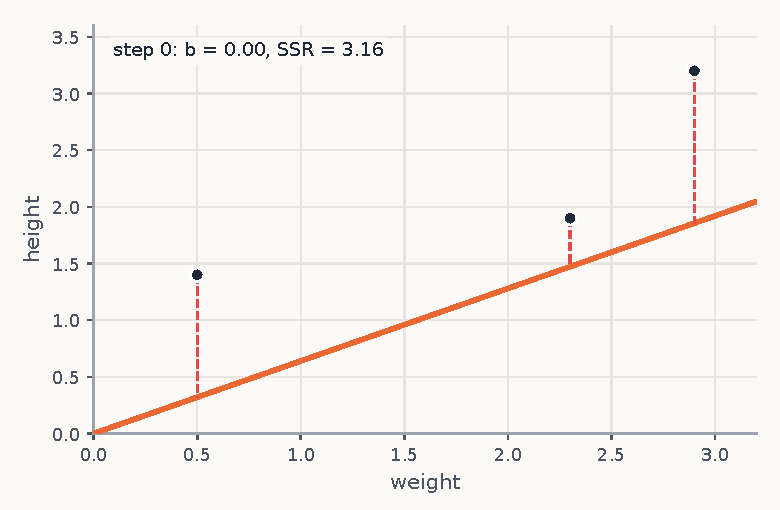
\includegraphics[width=\linewidth,height=0.55\textheight,keepaspectratio]{fig_line_frame_0}}%
      \only<2>{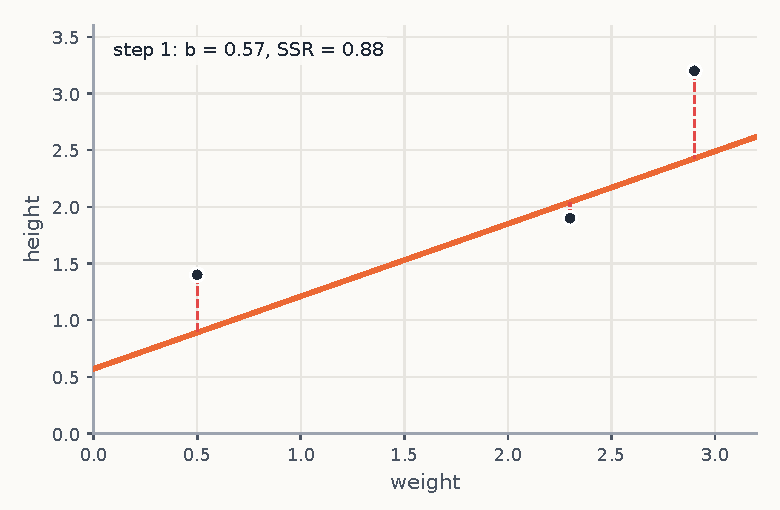
\includegraphics[width=\linewidth,height=0.55\textheight,keepaspectratio]{fig_line_frame_1}}%
      \only<3>{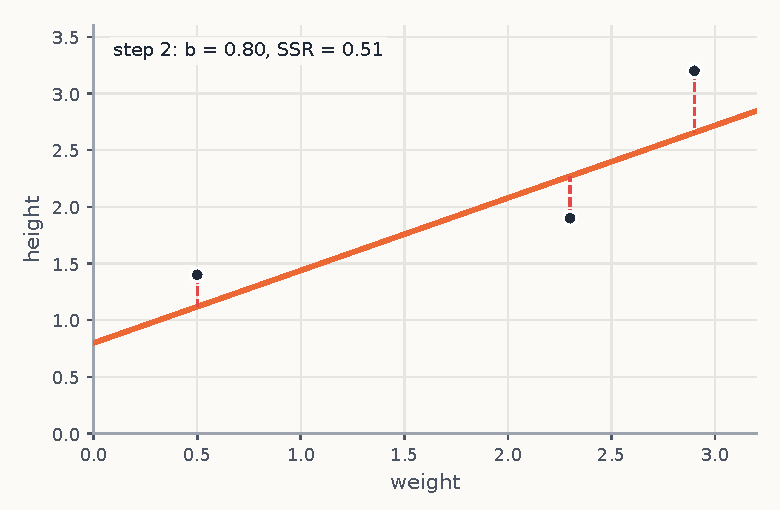
\includegraphics[width=\linewidth,height=0.55\textheight,keepaspectratio]{fig_line_frame_2}}%
      \only<4>{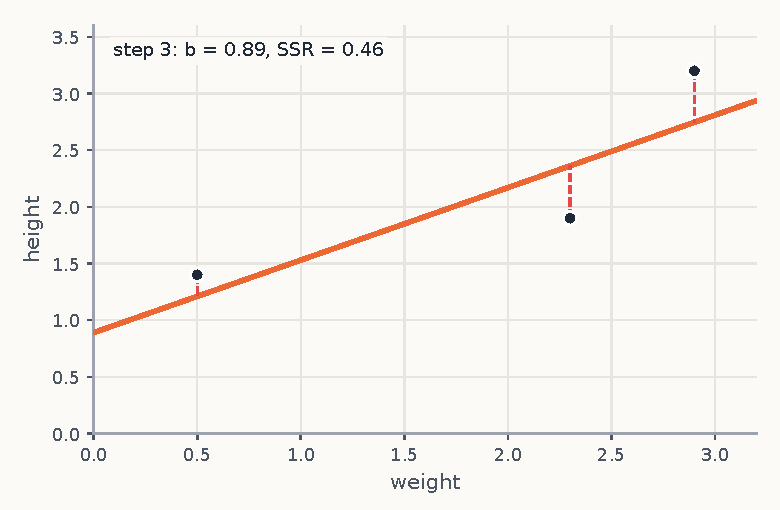
\includegraphics[width=\linewidth,height=0.55\textheight,keepaspectratio]{fig_line_frame_3}}%
      \only<5>{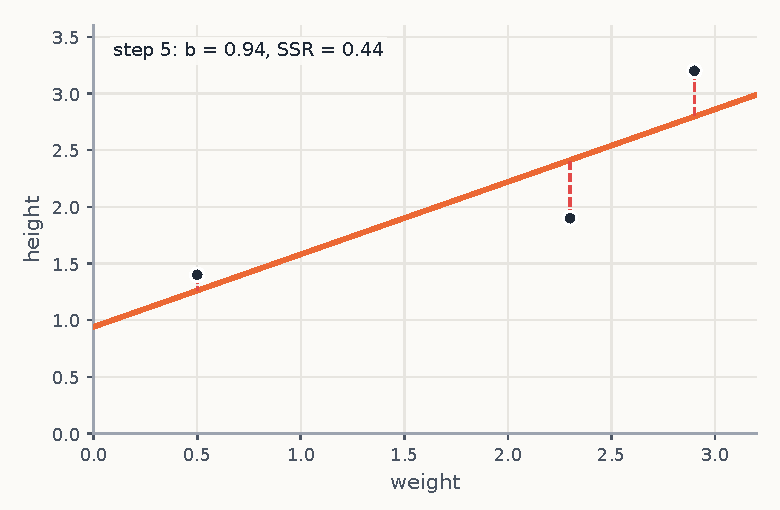
\includegraphics[width=\linewidth,height=0.55\textheight,keepaspectratio]{fig_line_frame_4}}%
      \only<6>{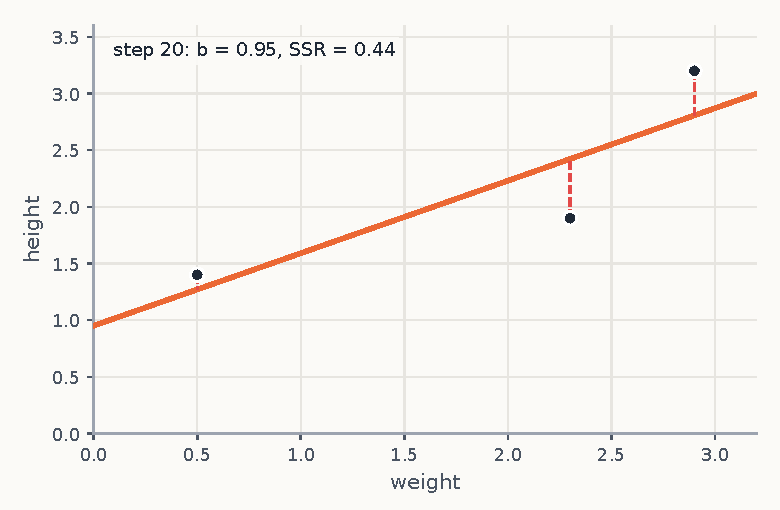
\includegraphics[width=\linewidth,height=0.55\textheight,keepaspectratio]{fig_line_frame_5}}%

      \footnotesize Data: weights $0.5, 2.3, 2.9$, heights $1.4, 1.9, 3.2$. Each click shows smaller residuals.
    \end{column}
  \end{columns}
\end{frame}

\begin{frame}{Why not just set the slope of the loss to zero?}
  \begin{columns}[T]
    \begin{column}{0.48\textwidth}
      \small
      At the best value the loss is flat, so solve loss$'=0$. For a line we \emph{can} (least squares).
      But often we \alert{cannot}: there is no closed form (logistic regression, neural nets),
      there are millions of parameters, or new data keeps arriving.
      \begin{thmbox}[The idea of gradient descent]
        \footnotesize Start from a guess and step downhill until the loss stops improving:
        \alert{big steps} far away, \alert{small steps} near the optimum.
        Cauchy proposed it in 1847~\cite{cauchy1847}; it is still used to train large models~\cite{bottou2018}.
      \end{thmbox}
    \end{column}
    \begin{column}{0.5\textwidth}
      \centering
      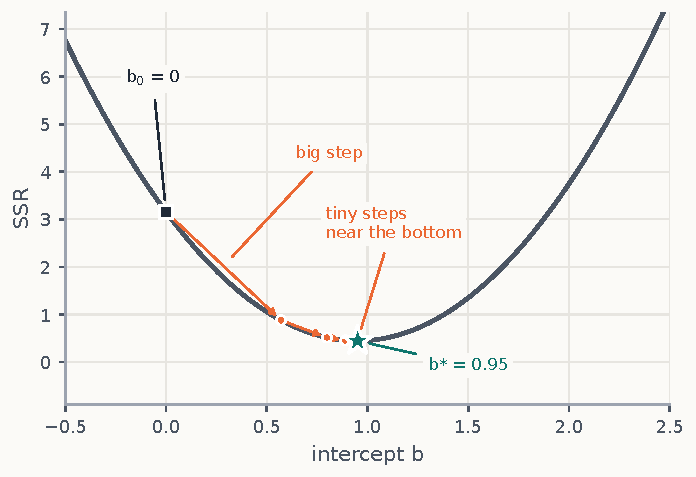
\includegraphics[width=\linewidth, height=0.55\textheight, keepaspectratio]{fig_ssr_intercept}

      \footnotesize SSR against the intercept (slope $0.64$). Steps shrink as the slope flattens.
    \end{column}
  \end{columns}
\end{frame}

% =====================================================================
%  2. The gradient: direction of steepest slope
% =====================================================================
\section{The gradient: direction of steepest slope}

\begin{frame}{From derivative to gradient}
  \begin{columns}[T]
    \begin{column}{0.5\textwidth}
      \small
      One variable: $J'(x)$ is the slope. Several: stack the partial derivative for \alert{each} variable,
      \[
        \nabla J(\x) = \begin{pmatrix}\partial J/\partial x_1\\ \vdots \\ \partial J/\partial x_n\end{pmatrix}.
      \]
      Example: $J = x_1^2 + x_2^2$ gives $\nabla J = (2x_1,\ 2x_2)$.

      \begin{keybox}[What the gradient tells us]
        \footnotesize At every point, $\nabla J$ is a vector that gives the \textbf{direction} and the \textbf{size} of the steepest
        slope. Moving along $-\nabla J$ goes downhill fastest.
      \end{keybox}
    \end{column}
    \begin{column}{0.48\textwidth}
      \centering
      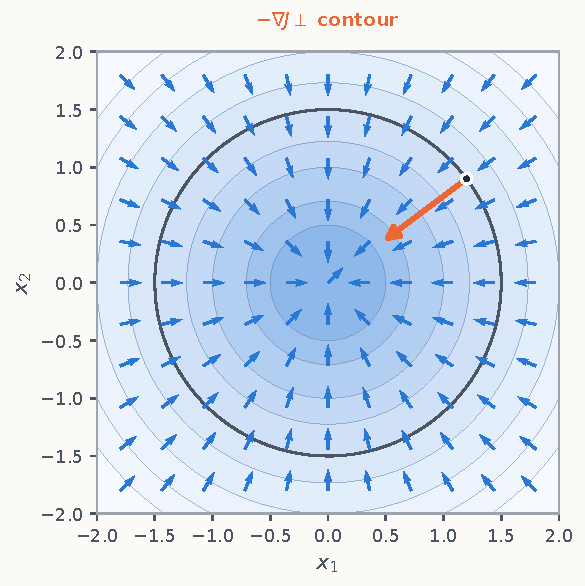
\includegraphics[width=\linewidth,height=0.56\textheight,keepaspectratio]{fig_gradient_field}

      \footnotesize Arrows: $-\nabla J$ on $J = x_1^2 + x_2^2$, pointing towards the minimum.
    \end{column}
  \end{columns}
\end{frame}

\begin{frame}{Why $-\nabla J$ is the steepest way down}
  \begin{columns}[T]
    \begin{column}{0.55\textwidth}
      \small
      Take a small step $t$ in a unit direction $\vd$. By Taylor,
      $J(\x + t\vd) \approx J(\x) + t\,\nabla J(\x)\T\vd$, so the rate of change along $\vd$ is
      $\nabla J\T\vd$.
      \begin{thmbox}[Claim]
        Among all unit directions, $\nabla J\T\vd$ is smallest at $\vd^\star = -\nabla J/\norm{\nabla J}$,
        where it equals $-\norm{\nabla J}$.
      \end{thmbox}
      \textbf{Proof.} By Cauchy--Schwarz, $|\nabla J\T\vd|\le\norm{\nabla J}\norm{\vd} = \norm{\nabla J}$, so
      $\nabla J\T\vd\ge-\norm{\nabla J}$. Equality holds when $\vd$ parallel to $\nabla J$, pointing the opposite way. $\blacksquare$

      \vspace{3pt}
      \footnotesize This identifies the direction of steepest descent~\cite{boyd2004,cauchy1847}.
    \end{column}
    \begin{column}{0.43\textwidth}
      \centering
      % Steepest-descent geometry: the half-plane of descent directions, the unit
% circle of candidate directions d, the gradient and the angle theta.
\begin{tikzpicture}[scale=1.4, >={Stealth[length=7pt]}]
  % descent half-plane  {d : grad^T d < 0}  (gradient direction (0.447, 0.894))
  \begin{scope}
    \clip (-1.75,-1.35) rectangle (1.75,1.35);
    \fill[mGreen!9] (-2,1) -- (2,-1) -- (2,-3) -- (-2,-3) -- cycle;
  \end{scope}
  \draw[mGrey, dashed, line width=0.6pt] (-1.75,0.875) -- (1.75,-0.875);
  \node[font=\scriptsize, mGreen, anchor=south east] at (1.60,-1.23) {descent directions};
  \node[font=\scriptsize, mGrey, rotate=-26.6, anchor=south west] at (-1.72,0.94) {level set};
  % unit circle
  \draw[mDarkTeal!35, line width=1pt] (0,0) circle (1);
  % candidate directions (faint)
  \foreach \t in {200,230,260,290,320,350,80,110,140,170}
    \draw[mGrey!45, -{Stealth[length=4pt]}] (0,0) -- (\t:1);
  % a generic direction d and the angle
  \draw[->, line width=1.3pt, mBlue] (0,0) -- (-15:1) node[right, font=\small] {$\vd$};
  \draw[mBlue, line width=0.7pt] (63.4:0.43) arc[start angle=63.4, end angle=-15, radius=0.43];
  \node[mBlue, font=\small] at (24:0.67) {$\theta$};
  % gradient and steepest descent
  \draw[->, line width=1.8pt, mRed] (0,0) -- (63.4:1.18) node[above, font=\small] {$\nabla f(\x)$};
  \draw[->, line width=1.8pt, mGreen] (0,0) -- (243.4:1) node[below left=3pt, font=\small] {$\vd^\star$};
  \fill[mInk] (0,0) circle (1.4pt);
  \node[font=\small, mInk, fill=mPaper, inner sep=1pt] at (-0.28,0.27) {$\x$};
\end{tikzpicture}


      \footnotesize The rate along $\vd$ is $\norm{\nabla J}\cos\theta$, lowest at $\theta = 180^\circ$.
    \end{column}
  \end{columns}
\end{frame}

\begin{frame}{Contour plots, and why GD crosses them at right angles}
  \begin{columns}[T]
    \begin{column}{0.5\textwidth}
      \small
      A contour plot draws $J(x_1, x_2)$ as rings of equal height.

      \textbf{Why $\nabla J\perp$ contour.} Move along a contour by a small $\mathbf t$; the height does not change:
      \[
        J(\x + \mathbf t) - J(\x)\approx\nabla J\T\mathbf t = 0 .
      \]
      So each GD step leaves its contour at a right angle.
      \begin{keybox}[Reading a contour plot]
        \footnotesize Close contours: steeper slopes, larger steps. Wide gaps: smaller steps.
      \end{keybox}
    \end{column}
    \begin{column}{0.48\textwidth}
      \centering
      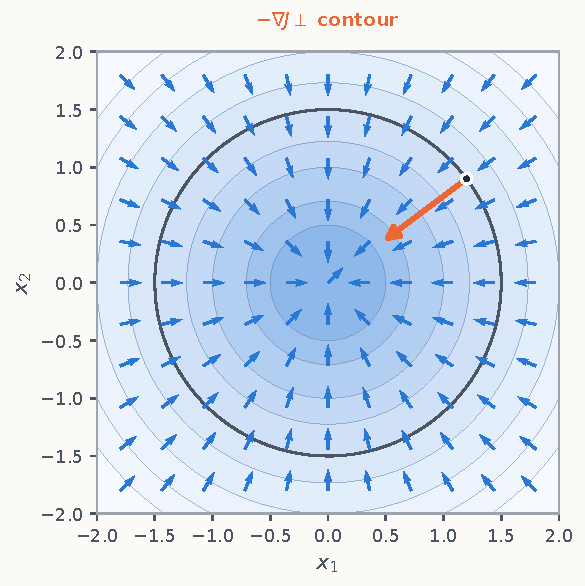
\includegraphics[width=\linewidth,height=0.7\textheight,keepaspectratio]{fig_gradient_field}
    \end{column}
  \end{columns}
\end{frame}

\begin{frame}{When the gradient is zero}
  \small
  Setting $\nabla J = \mathbf 0$ finds \emph{stationary} points. The second derivative tells them apart:

  \vspace{4pt}
  \centering
  \begin{tabular}{@{}l l l l@{}}
    \toprule
    Function & Stationary point & Second derivative & Type \\
    \midrule
    $J = x^2$ & $J' = 2x = 0\Rightarrow x = 0$ & $J'' = 2 > 0$ & \textcolor{mTeal}{\textbf{minimum}} \\
    $J = -x^2$ & $x = 0$ & $J'' = -2 < 0$ & \textcolor{mOrange}{\textbf{maximum}} \\
    $J = x^3$ & $J' = 3x^2 = 0\Rightarrow x = 0$ & $J'' = 6x = 0$, sign changes & \textcolor{mRed}{\textbf{saddle}} \\
    $J = x_1^2 + x_2^2$ & $\nabla J = (2x_1, 2x_2) = \mathbf 0$ & both curvatures $2 > 0$ & \textcolor{mTeal}{\textbf{minimum}} at $(0,0)$ \\
    \bottomrule
  \end{tabular}

  \vspace{6pt}
  \raggedright
  \begin{warnbox}[Zero gradient is not the same as a minimum]
    GD stops wherever the gradient vanishes, so it can stall at a saddle or settle in a \emph{local} minimum.
    Problem M1 shows this on the quartic $J = x^4 - 6x^3 + 8x^2$.
  \end{warnbox}
\end{frame}

\begin{frame}{What the three kinds of point look like}
  \begin{columns}[T]
    \begin{column}{0.5\textwidth}
      \centering
      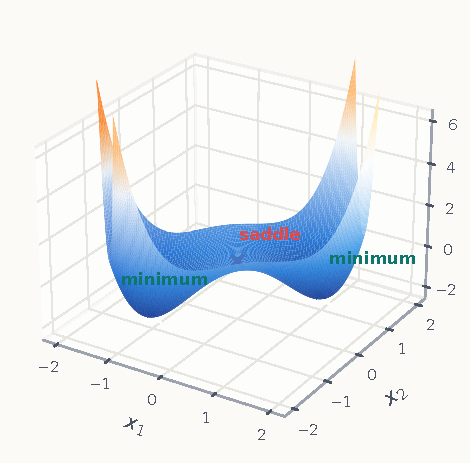
\includegraphics[width=\linewidth, height=0.62\textheight, keepaspectratio]{fig_quartic_surface}
    \end{column}
    \begin{column}{0.48\textwidth}
      \centering
      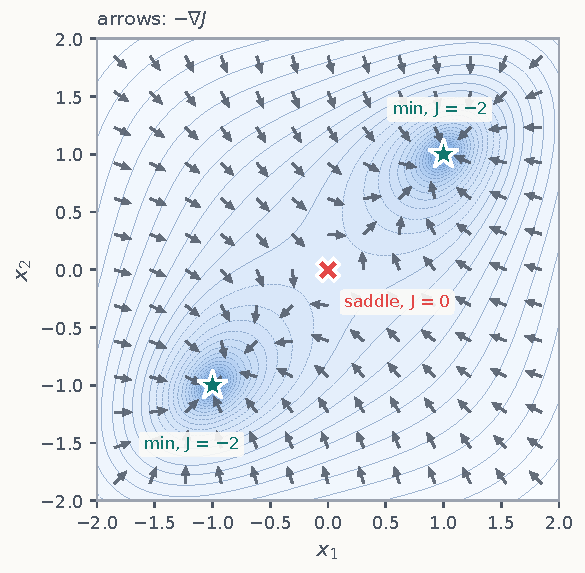
\includegraphics[width=\linewidth, height=0.62\textheight, keepaspectratio]{fig_quartic_contour}
    \end{column}
  \end{columns}
  \vspace{2pt}
  \footnotesize $J = x_1^4 + x_2^4 - 4x_1x_2$ has $\nabla J = \mathbf 0$ at three points: two \textcolor{mTeal}{\textbf{minima}}
  at $\pm(1, 1)$ and a \textcolor{mRed}{\textbf{saddle}} at the origin. The arrows ($-\nabla J$) flow into the valleys,
  and at the saddle they arrive along one direction and leave along the other.
\end{frame}

% =====================================================================
%  3. The update rule: step = slope \times learning rate
% =====================================================================
\section{The update rule: step = slope $\times$ learning rate}

\begin{frame}{One parameter: the running example, with numbers}
  \small
  Fix the slope at $m = 0.64$ and let GD find the intercept $b$, starting from $b_0 = 0$ with learning rate $\alpha = 0.1$.
  \[
    \frac{d\,\SSR}{db} = -2\sum_{i}\bigl(y_i - b - 0.64\,x_i\bigr),\quad
    \text{step} = \frac{d\,\SSR}{db}\times\alpha,\quad b_{\text{new}} = b_{\text{old}} - \text{step}.
  \]
  \centering\footnotesize
  \begin{tabular}{@{}c c c c c@{}}
    \toprule
    step $k$ & $b_k$ & slope $d\SSR/db$ & step size & $\SSR(b_{k+1})$ \\
    \midrule
    0 & $0$ & $-5.704$ & $-0.5704$ & $0.878$ \\
    1 & $0.5704$ & $-2.282$ & $-0.2282$ & $0.514$ \\
    2 & $0.7986$ & $-0.913$ & $-0.0913$ & $0.456$ \\
    3 & $0.8898$ & $-0.365$ & $-0.0365$ & $0.446$ \\
    \bottomrule
  \end{tabular}

  \raggedright
  \vspace{4pt}
  Each step is about $0.4\times$ the last (start $\SSR = 3.156$), and $b$ settles at \ans{b^\star = 0.951}.\par
  Steps shrink because the slope flattens near the minimum.
\end{frame}

\begin{frame}{Updating several parameters}
  \begin{columns}[T]
    \begin{column}{0.46\textwidth}
      \centering
      \scalebox{0.9}{% Gradient descent loop, steps (i)-(vi)
\begin{tikzpicture}[
  node distance=0.30cm,
  step/.style={draw=#1, line width=0.8pt, rounded corners=4pt, fill=white,
               drop shadow={opacity=0.15, shadow xshift=0.5pt, shadow yshift=-0.7pt},
               text width=3.8cm, minimum height=0.62cm, align=left, font=\scriptsize\color{mInk},
               inner xsep=10pt},
  step/.default=mNavy,
  badge/.style={circle, fill=#1, text=white, font=\tiny\bfseries, inner sep=1pt, minimum size=10pt},
  arr/.style={-{Stealth[length=5pt]}, line width=0.9pt, mGrey}]
  \node[step] (s1) {take the derivative of the loss for each parameter};
  \node[step, below=of s1] (s2) {pick a starting value for each parameter};
  \node[step, below=of s2] (s3) {plug the current values into the derivatives};
  \node[step=mOrange, below=of s3] (s4) {step size $=$ slope $\times$ learning rate};
  \node[step=mOrange, below=of s4] (s5) {new value $=$ old value $-$ step size};
  \node[step=mTeal, below=of s5] (s6) {stop if the step is tiny or max steps reached};
  \foreach \a/\b in {s1/s2, s2/s3, s3/s4, s4/s5, s5/s6} \draw[arr] (\a) -- (\b);
  \draw[arr] (s6.east) -- ++(0.55,0) |- node[pos=0.25, right=3pt, font=\scriptsize, mGrey] {not yet} (s3.east);
  \foreach \n/\lab/\c in {s1/i/mNavy, s2/ii/mNavy, s3/iii/mNavy, s4/iv/mOrange, s5/v/mOrange, s6/vi/mTeal}
    \node[badge=\c] at (\n.west) {\lab};
\end{tikzpicture}
}
    \end{column}
    \begin{column}{0.52\textwidth}
      \small
      For $\hat y = b + mx$ both parameters move:
      \begin{align*}
        \frac{\partial\SSR}{\partial b} &= -2\sum_i\bigl(y_i - b - m x_i\bigr),\\
        \frac{\partial\SSR}{\partial m} &= -2\sum_i x_i\bigl(y_i - b - m x_i\bigr).
      \end{align*}
      In general, for every $w_j$ at once:
      \[
        \ans{w_j \leftarrow w_j - \alpha\,\frac{\partial J}{\partial w_j}}
      \]
      \textbf{Stop} when the step size is near zero (say $<10^{-3}$) or after a maximum number of steps.
    \end{column}
  \end{columns}
\end{frame}

\begin{frame}{Where the update comes from: first-order Taylor}
  \begin{columns}[T]
    \begin{column}{0.52\textwidth}
      \small
      Newton uses a \emph{second}-order Taylor model. Use the \emph{first}-order one, trusted only near $\x_k$
      (constant $J(\x_k)$ dropped):
      \[
        \x_{k+1} = \argmin_{\x}\Bigl\{\underbrace{\nabla J(\x_k)\T(\x - \x_k)}_{\text{straight-line model}}
          + \underbrace{\tfrac{1}{2\alpha}\norm{\x - \x_k}^2}_{\text{stay close}}\Bigr\}.
      \]
      Setting the gradient of the braces to zero gives
      $\nabla J(\x_k) + \tfrac1\alpha(\x - \x_k) = \mathbf 0$, i.e.
      \[
        \ans{\x_{k+1} = \x_k - \alpha\,\nabla J(\x_k)}
      \]
      so the learning rate controls \alert{how far we trust the straight-line model}.
    \end{column}
    \begin{column}{0.46\textwidth}
      \centering
      \footnotesize
      \begin{tabular}{@{}l c c@{}}
        \toprule
        & GD & Newton \\
        \midrule
        Taylor model & 1st order & 2nd order \\
        uses & $\nabla J$ & $\nabla J$, Hessian $H$ \\
        update & $\x - \alpha\nabla J$ & $\x - H^{-1}\nabla J$ \\
        step length & set by $\alpha$ & set by curvature \\
        \bottomrule
      \end{tabular}

      \vspace{6pt}
      \raggedright\footnotesize Newton's method~\cite{chapra} offers another approach; Section 6 compares their costs.
    \end{column}
  \end{columns}
\end{frame}

\begin{frame}{Gradient descent as forward Euler}
  \small
  Let a point slide downhill in continuous time. The \textbf{gradient flow} ODE always lowers $J$:
  \[
    \dot\x(t) = -\nabla J(\x(t)) \quad\Longrightarrow\quad \frac{d}{dt}J(\x(t)) = \nabla J\T\dot\x = -\norm{\nabla J}^2 \le 0 .
  \]
  Solve it with \textbf{forward Euler}, step $h$~\cite{chapra}: $\;\x_{k+1} = \x_k + h\,(-\nabla J(\x_k))$.
  That is \alert{gradient descent with $\alpha = h$}, so Euler's stability analysis applies.

  \vspace{3pt}
  \centering\footnotesize
  \begin{tabular}{@{}l l@{}}
    \toprule
    Numerical ODEs & Optimisation \\
    \midrule
    Euler is stable only if $|1 - h\lambda| < 1$ & the learning-rate limit $\alpha < 2/f''$ (Section 5) \\
    stiff system (eigenvalues far apart) & stretched contours and the zig-zag (Section 4) \\
    implicit (backward) Euler & the proximal-point method, stable for any step \\
    a ball with mass and friction & momentum (Section 8) \\
    $\ddot\x + \tfrac3t\dot\x + \nabla J = 0$ & Nesterov's method~\cite{su2016} \\
    \bottomrule
  \end{tabular}
\end{frame}

\statement{THE ODE CONNECTION}{Gradient descent is forward Euler\\ on the gradient flow.}{So the learning-rate limit is a stability limit, and a stretched valley is a stiff ODE.}

\begin{frame}[fragile]{Many parameters at once: the vectorised update}
  \begin{columns}[T]
    \begin{column}{0.4\textwidth}
      \small
      Multiple linear regression~\cite{chapra}: $\hat y = w_0 + w_1x_1 + \dots + w_nx_n$ with the mean squared error
      \[
        J(\w) = \frac{1}{2m}\sum_{i=1}^{m}\bigl(\hat y_i - y_i\bigr)^2 .
      \]
      Stack a column of ones and the features into $\bX$. All partial derivatives come from one product,
      \[
        \nabla J(\w) = \tfrac1m\,\bX\T(\bX\w - \vy),
      \]
      so one step costs $O(mn)$: two matrix-vector products, no matrix inversion.
    \end{column}
    \begin{column}{0.58\textwidth}
\begin{lstlisting}[style=py]
import numpy as np

def gd(X, y, alpha=0.1, tol=1e-8,
       steps=10_000):
    X = np.column_stack([np.ones(len(y)), X])
    w = np.zeros(X.shape[1])            # (ii)
    for k in range(steps):
        g = X.T @ (X @ w - y) / len(y)  # (iii)
        step = alpha * g                # (iv)
        w = w - step                    # (v)
        if np.linalg.norm(step) < tol:  # (vi)
            break
    return w, k
\end{lstlisting}
      \footnotesize The comments match steps (i)--(vi) of the loop.
    \end{column}
  \end{columns}
\end{frame}

% =====================================================================
%  4. Watching it move
% =====================================================================
\section{Watching it move}

\begin{frame}{Gradient descent, one step at a time}
  \centering
  \only<1>{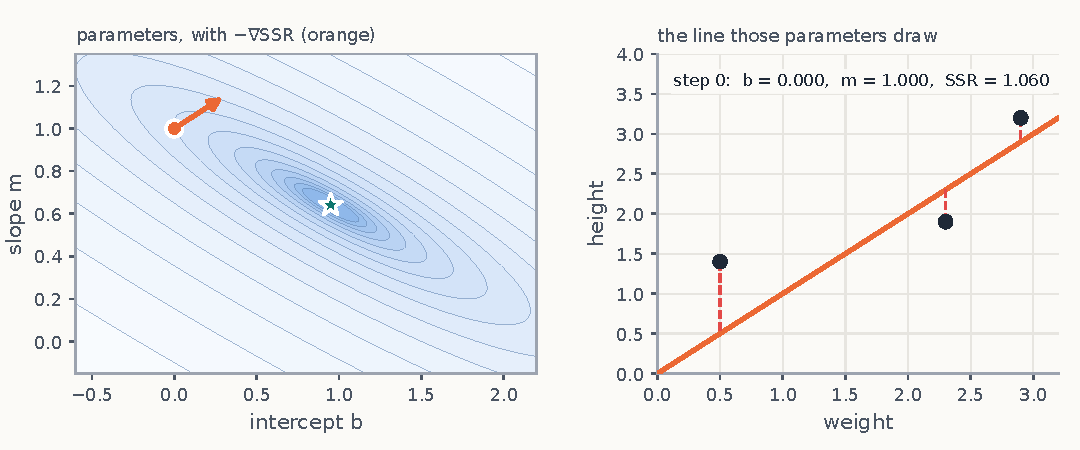
\includegraphics[width=\textwidth, height=0.6\textheight, keepaspectratio]{fig_ssr_frame_0}}%
  \only<2>{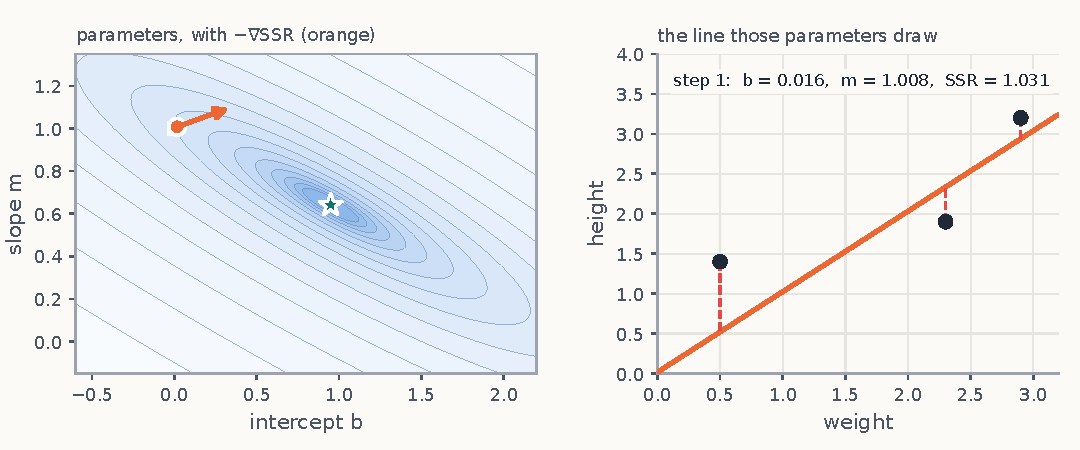
\includegraphics[width=\textwidth, height=0.6\textheight, keepaspectratio]{fig_ssr_frame_1}}%
  \only<3>{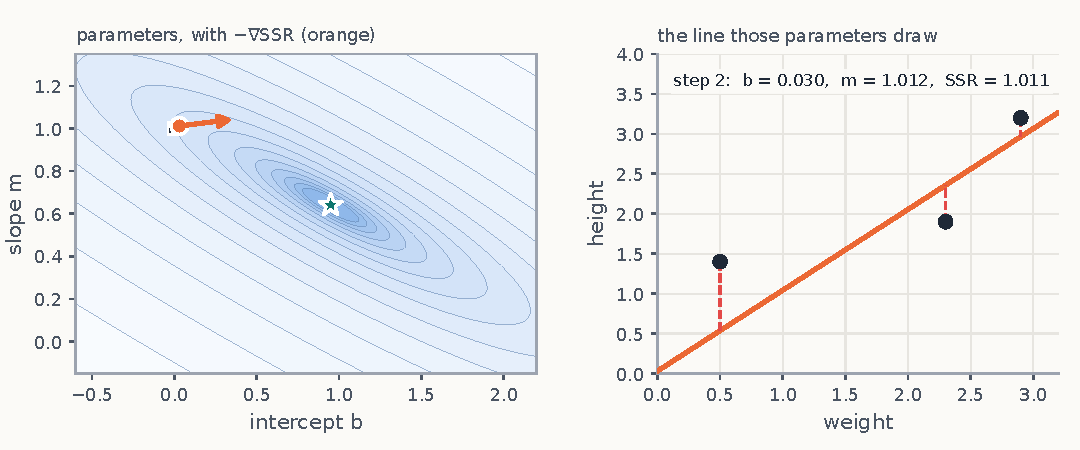
\includegraphics[width=\textwidth, height=0.6\textheight, keepaspectratio]{fig_ssr_frame_2}}%
  \only<4>{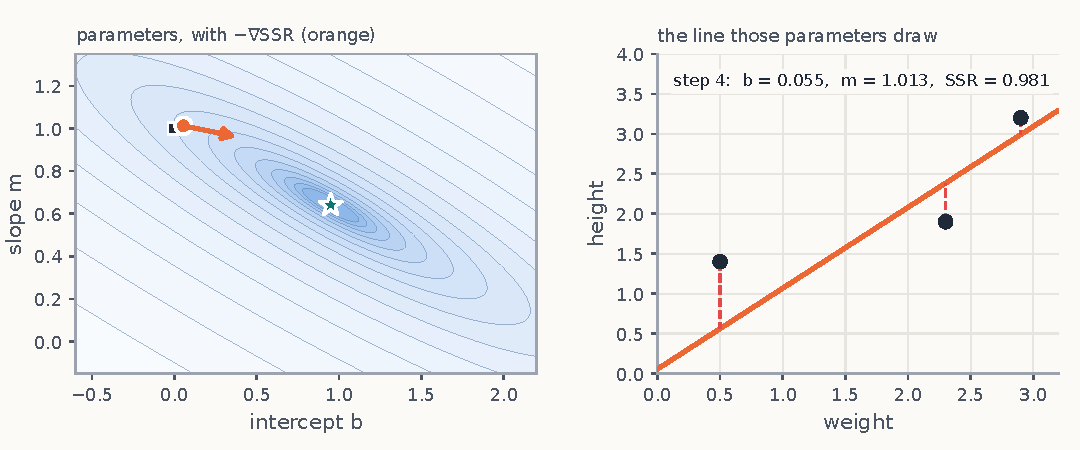
\includegraphics[width=\textwidth, height=0.6\textheight, keepaspectratio]{fig_ssr_frame_3}}%
  \only<5>{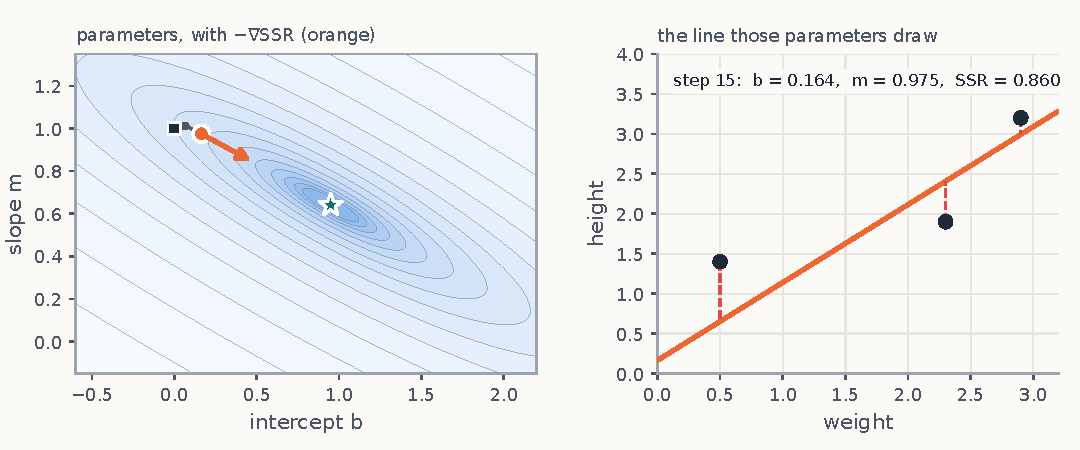
\includegraphics[width=\textwidth, height=0.6\textheight, keepaspectratio]{fig_ssr_frame_4}}%
  \only<6>{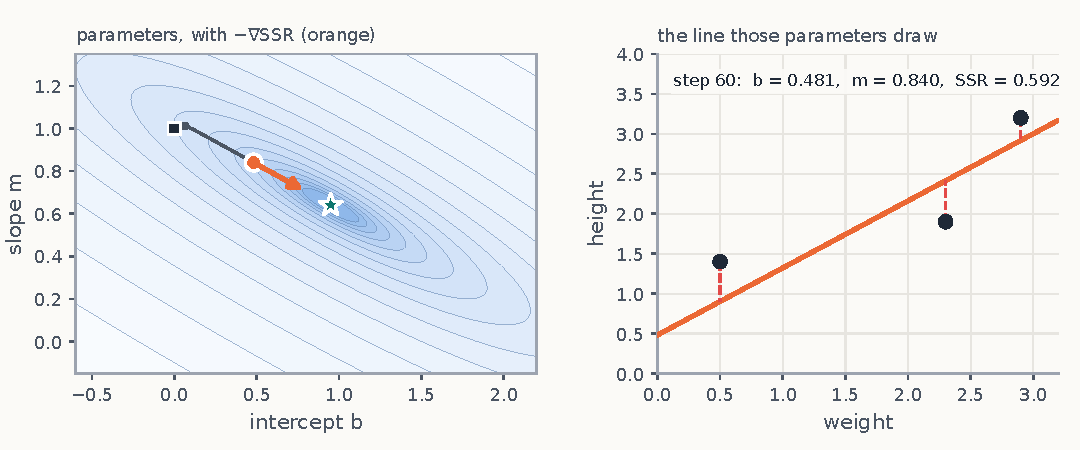
\includegraphics[width=\textwidth, height=0.6\textheight, keepaspectratio]{fig_ssr_frame_5}}%
  \only<7>{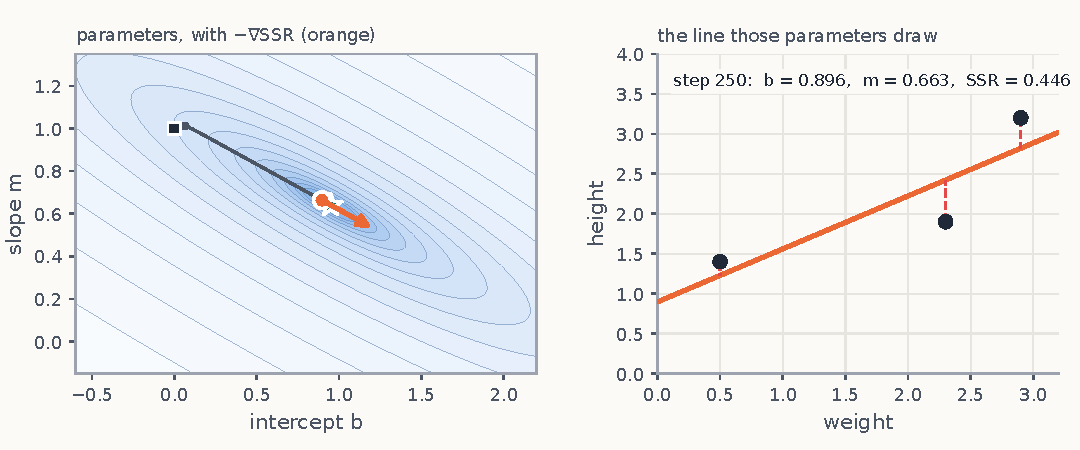
\includegraphics[width=\textwidth, height=0.6\textheight, keepaspectratio]{fig_ssr_frame_6}}%
  \only<8>{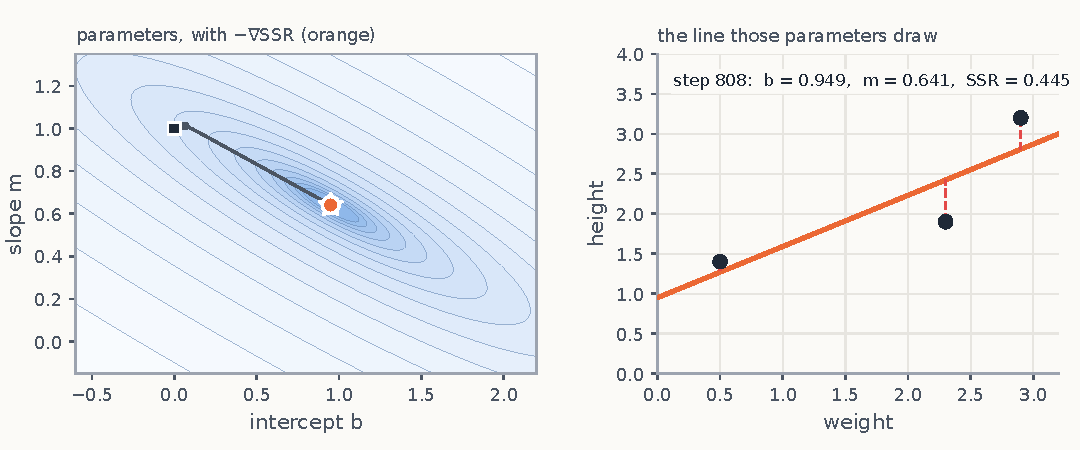
\includegraphics[width=\textwidth, height=0.6\textheight, keepaspectratio]{fig_ssr_frame_7}}%

  \raggedright\footnotesize
  Weight--height data, both parameters free, $\alpha = 0.01$ from $(b, m) = (0, 1)$, as in Problem A1.
  Left: the point $(b, m)$ walks downhill across the SSR contours. Right: the line that point draws.
  Click through steps $0, 1, 2, 4, 15, 60, 250, 808$.
\end{frame}

\begin{frame}{The same walk on the SSR surface}
  \begin{columns}[T]
    \begin{column}{0.56\textwidth}
      \centering
      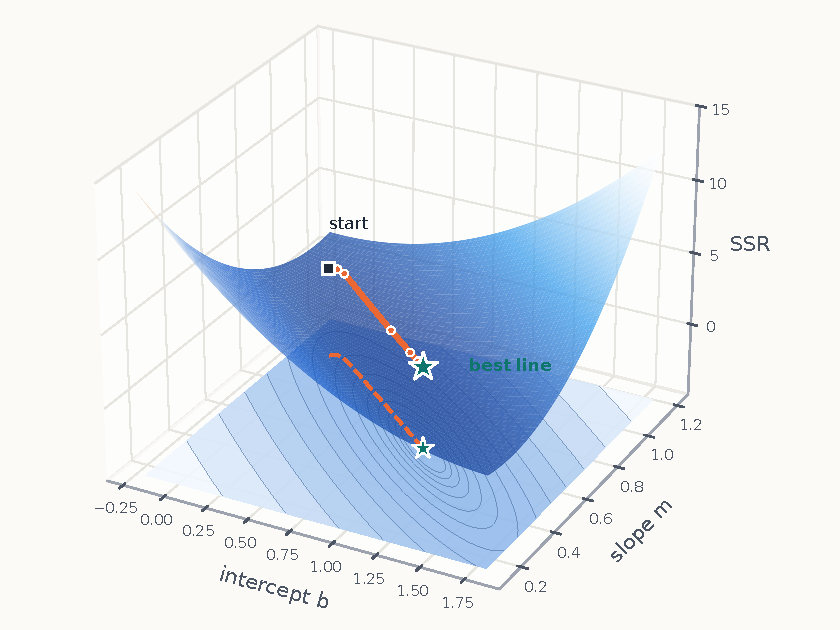
\includegraphics[width=\linewidth, height=0.76\textheight, keepaspectratio]{fig_ssr_surface}
    \end{column}
    \begin{column}{0.42\textwidth}
      \small
      $\SSR(b, m)$ is a bowl over the $(b, m)$ plane. Every point of the bowl is one line through the data.
      \begin{itemize}\footnotesize
        \item GD starts at $(0, 1)$ and rolls downhill. The dashed curve is its shadow on the contour map,
              the path of the previous slide.
        \item It drops into the valley in a few steps, then creeps along the valley floor, because the valley
              is long and narrow ($\kappa \approx 29$, Section 7).
        \item After $808$ steps it stops at $(0.9486,\ 0.6411)$, the least-squares line $(0.9487,\ 0.6410)$.
      \end{itemize}
    \end{column}
  \end{columns}
\end{frame}

\begin{frame}{Stretched contours make GD zig-zag}
  \centering
  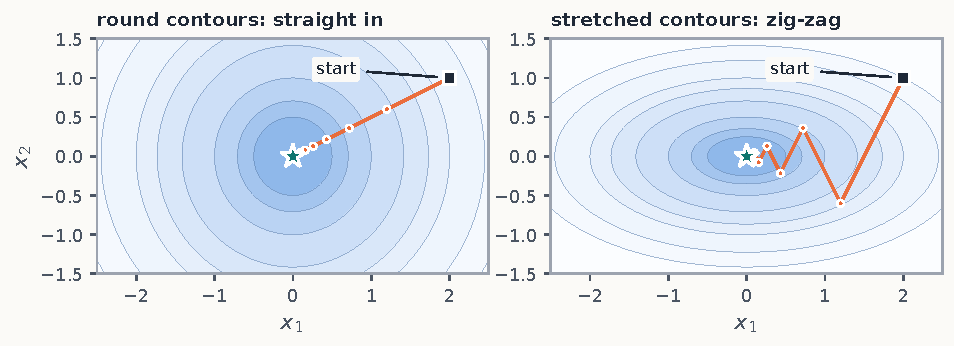
\includegraphics[width=\textwidth,height=0.42\textheight,keepaspectratio]{fig_zigzag_scaling}

  \raggedright
  \footnotesize
  \begin{itemize}
    \item Round rings ($x_1^2 + x_2^2$): $-\nabla J$ points straight at the minimum.
    \item Stretched rings ($x_1^2 + 4x_2^2$): it points across the valley; GD zig-zags. The steep
          direction ($f'' = 8$) caps $\alpha < 2/8$; the flat one ($f'' = 2$) then needs many steps.
    \item \textbf{Fix: scale the features} to similar curvature (standardise inputs, Problem A2).
  \end{itemize}
\end{frame}

% =====================================================================
%  5. How big a step? When GD works
% =====================================================================
\section{How big a step? When GD works}

\begin{frame}{Learning rate and the path}
  \begin{columns}[T]
    \begin{column}{0.6\textwidth}
      \centering
      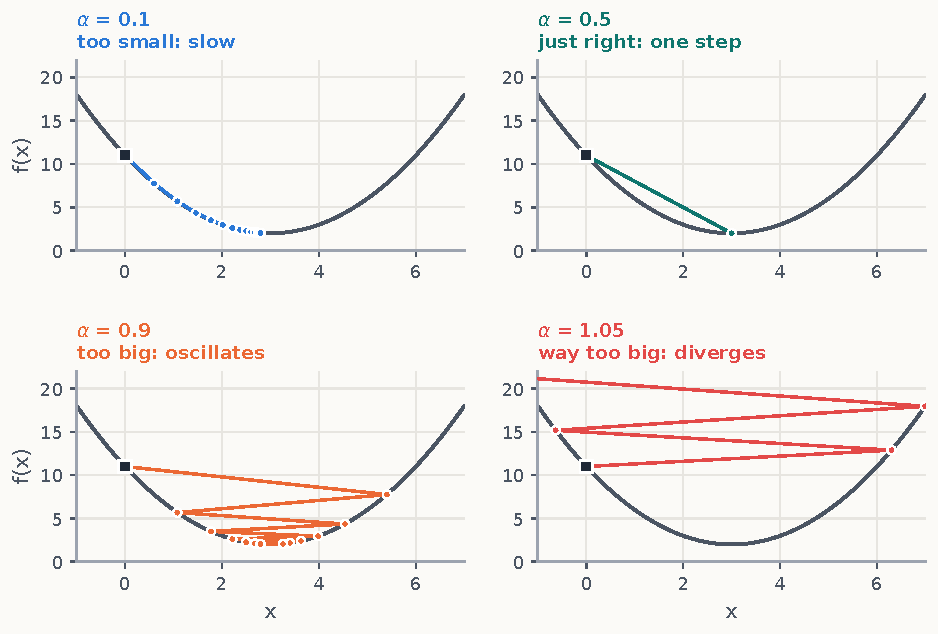
\includegraphics[width=\linewidth, height=0.78\textheight, keepaspectratio]{fig_lr_regimes}
    \end{column}
    \begin{column}{0.38\textwidth}
      \small
      GD on $f(x) = (x-3)^2 + 2$ from $x_0 = 0$ with four learning rates:
      \begin{itemize}\footnotesize
        \item $\alpha = 0.1$: every step goes the right way, but slowly.
        \item $\alpha = 0.5$: lands on $x = 3$ in \emph{one} step.
        \item $\alpha = 0.9$: jumps over the minimum each time, but still closes in.
        \item $\alpha = 1.05$: each jump is bigger than the last. It \alert{diverges}.
      \end{itemize}
      \footnotesize\textcolor{mGrey}{Same function, same start: only $\alpha$ changed.}
    \end{column}
  \end{columns}
\end{frame}

\begin{frame}{Exactly when does GD converge?}
  \small
  For $f(x) = (x-3)^2 + 2$: $f'(x) = 2(x-3)$. Write the error as $e_k = x_k - 3$:
  \[
    x_{k+1} = x_k - 2\alpha(x_k - 3) \quad\Longrightarrow\quad \ans{e_{k+1} = (1 - 2\alpha)\,e_k}
    \quad\Longrightarrow\quad e_k = (1-2\alpha)^k e_0 .
  \]
  \centering\footnotesize
  \begin{tabular}{@{}l c l@{}}
    \toprule
    learning rate & factor $1 - 2\alpha$ & what happens \\
    \midrule
    $0 < \alpha < 0.5$ & between $0$ and $1$ & steady approach from one side \\
    $\alpha = 0.5$ & $0$ & exact in one step \\
    $0.5 < \alpha < 1$ & between $-1$ and $0$ & overshoots, oscillates inwards \\
    $\alpha > 1$ & below $-1$ & \textcolor{mRed}{\textbf{diverges}} \\
    \bottomrule
  \end{tabular}

  \raggedright
  \vspace{4pt}
  \begin{keybox}[The general rule]
    \footnotesize With curvature $f'' > 0$ the error factor is $1 - \alpha f''$, so GD is stable only if
    $\ans{0 < \alpha < 2/f''}$; best fixed step $\alpha = 1/f''$. Running example: $f'' = 6$, so $\alpha < 1/3$, and
    $\alpha = 0.1$ gives factor $0.4$, the shrink in the table.
  \end{keybox}
\end{frame}

\begin{frame}{Euler's stability region explains the learning-rate limit}
  \begin{columns}[T]
    \begin{column}{0.52\textwidth}
      \small
      Take $J = x_1^2 + 4x_2^2$ (Problem M3). Its curvatures are $\lambda = 2$ and $8$, and each direction
      is the test equation $\dot y = -\lambda y$.
      \begin{itemize}\footnotesize
        \item The \textbf{exact flow} decays for every $\lambda > 0$: the continuous system is stable.
        \item \textbf{Forward Euler} multiplies $y$ by $1 + z$ with $z = -\alpha\lambda$. It is stable only inside the disk
              $|1 + z| < 1$, i.e.\ $\alpha < 2/\lambda$ for \emph{every} $\lambda$: $\alpha < 2/8$.
        \item This is \textbf{stiffness}: the steepest direction caps the step, the flattest one slows convergence.
      \end{itemize}
    \end{column}
    \begin{column}{0.46\textwidth}
      \centering
      % Forward-Euler stability disk |1 + z| < 1 with the points z_i = -alpha*lambda_i
% for J = x1^2 + 4 x2^2 (lambda = 2, 8): alpha = 0.1 (stable) and alpha = 0.3 (unstable)
\begin{tikzpicture}[scale=1.3, >={Stealth[length=5pt]}]
  \shade[inner color=mTeal!26, outer color=mTeal!5] (-1,0) circle (1);
  \draw[line width=1.1pt, mTeal] (-1,0) circle (1);
  \draw[->, mGrey] (-2.85,0) -- (0.6,0) node[right, font=\scriptsize] {$\mathrm{Re}\,z$};
  \draw[->, mGrey] (0,-1.2) -- (0,1.25) node[above, font=\scriptsize] {$\mathrm{Im}\,z$};
  \foreach \t/\lab in {-2/-2, -1/-1} {
    \draw[mGrey] (\t,0.05) -- (\t,-0.05);
    \node[font=\tiny, mGrey, anchor=north east, inner sep=1pt] at ({\t-0.06},-0.13) {$\lab$};
  }
  \node[font=\tiny, mGrey, anchor=north west, inner sep=2pt] at (0,-0.10) {$0$};
  \node[font=\scriptsize\bfseries, mTeal] at (-1,0.55) {stable};
  % alpha = 0.1: z = -0.2, -0.8
  \fill[mBlue, draw=white, line width=0.6pt] (-0.2,0) circle (2.3pt);
  \fill[mBlue, draw=white, line width=0.6pt] (-0.8,0) circle (2.3pt);
  % alpha = 0.3: z = -0.6, -2.4
  \draw[mRed, line width=1.1pt, fill=white] (-0.6,0) circle (2.6pt);
  \draw[mRed, line width=1.1pt, fill=white] (-2.4,0) circle (2.6pt);
  \draw[mRed, ->] (-2.4,-0.62) node[below, font=\tiny] {escapes} -- (-2.4,-0.12);
\end{tikzpicture}


      \footnotesize
      \textcolor{mBlue}{$\bullet$} $\alpha = 0.1$: $z = -0.2, -0.8$, both inside.\\
      \textcolor{mRed}{$\circ$} $\alpha = 0.3$: $z = -0.6, -2.4$, one is outside.
    \end{column}
  \end{columns}
\end{frame}

\begin{frame}{The stable window and the best fixed step}
  \begin{columns}[T]
    \begin{column}{0.5\textwidth}
      \begin{thmbox}[Theorem (quadratics)~\cite{nocedal2006}]
        \small With curvatures $\lmin \le \lambda_i \le \lmax$, GD converges from every start iff $0 < \alpha < 2/\lmax$, with rate
        \[
          \rho(\alpha) = \max\{|1 - \alpha\lmin|,\ |1 - \alpha\lmax|\}.
        \]
        The best step is $\alpha^\star = \frac{2}{\lmin + \lmax}$, giving $\rho^\star = \frac{\kappa - 1}{\kappa + 1}$, $\kappa = \frac{\lmax}{\lmin}$.
      \end{thmbox}
      \footnotesize\textbf{Proof.} $|1 - \alpha\lambda|$ is largest at an end of $[\lmin, \lmax]$; the best $\alpha$ makes the
      two ends equal, $1 - \alpha\lmin = \alpha\lmax - 1$. $\blacksquare$
    \end{column}
    \begin{column}{0.48\textwidth}
      \centering
      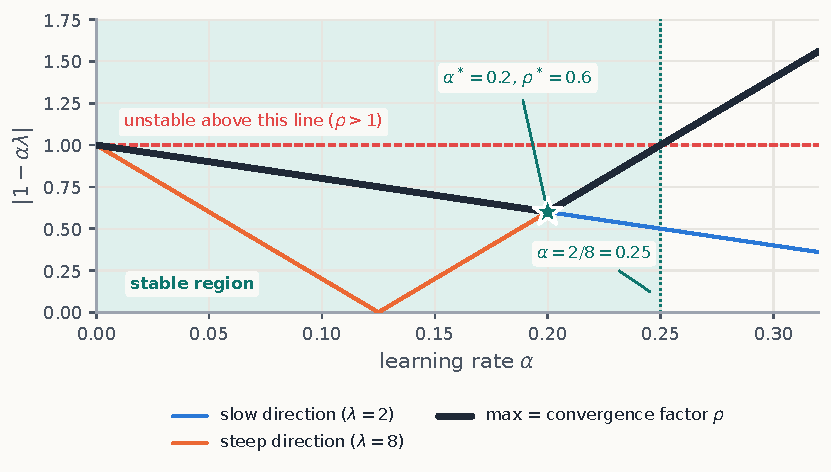
\includegraphics[width=\linewidth, height=0.5\textheight, keepaspectratio]{fig_stability_window}

      \footnotesize For M3: $\alpha^\star = 2/10 = 0.2$ and $\rho^\star = 3/5 = 0.6$. Close to a minimum every smooth $J$
      looks like a quadratic, so this describes GD near the minimum.
    \end{column}
  \end{columns}
\end{frame}

\statement{THE LEARNING RATE}{The learning rate controls\\ whether GD converges.}{Below $2/f''$ it converges. Above it, the error grows.}

% =====================================================================
%  6. How fast does it converge?
% =====================================================================
\section{How fast does it converge?}

\begin{frame}{Order of convergence: GD is linear}
  \begin{columns}[T]
    \begin{column}{0.5\textwidth}
      \small
      Near a minimum GD behaves like $e_{k+1}\approx\rho\,e_k$ with $\rho = |1 - \alpha f''|$: the error shrinks by the
      \alert{same factor} every step. That is \textbf{linear} convergence (order $p = 1$).

      To cut the error by $10^{6}$ we need $\rho^k\le10^{-6}$:
      \[
        k \ge \frac{\ln 10^{6}}{\ln(1/\rho)} .
      \]
      \begin{itemize}\footnotesize
        \item $f = (x-3)^2$, $\alpha = 0.1$: $\rho = 0.8$, so $k = \ans{62}$ steps.
        \item running example, $\alpha = 0.1$: $\rho = 0.4$, so $k = \ans{16}$ steps.
      \end{itemize}
      Newton is \textbf{quadratic} ($p = 2$): correct digits roughly double each step.
    \end{column}
    \begin{column}{0.48\textwidth}
      \centering
      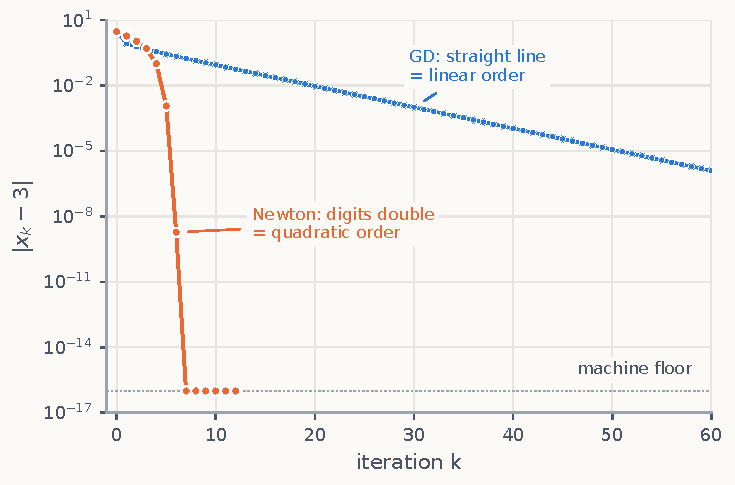
\includegraphics[width=\linewidth, height=0.56\textheight, keepaspectratio]{fig_gd_vs_newton}

      \footnotesize Log scale: linear falls steadily; quadratic falls faster
    \end{column}
  \end{columns}
\end{frame}

\begin{frame}{GD or Newton? Count the cost}
  \small
  \emph{When GD, and when Newton?} Count the work for $n$ parameters~\cite{nocedal2006}.

  \vspace{2pt}
  \centering\footnotesize
  \begin{tabular}{@{}l l l@{}}
    \toprule
    & Gradient descent & Newton's method \\
    \midrule
    information used & gradient ($n$ numbers) & gradient + Hessian ($n^2$ numbers) \\
    cost of one step & $O(n)$ after the gradient & $O(n^3)$ to solve $H\mathbf y = \g$ \\
    order of convergence & linear & quadratic \\
    learning rate & must be chosen & not needed \\
    on a concave stretch ($f'' < 0$) & still goes downhill & can head for a \textcolor{mRed}{maximum} \\
    best for & large problems (ML, $n\sim10^6$) & small problems needing high accuracy \\
    \bottomrule
  \end{tabular}

  \raggedright
  \vspace{3pt}
  \begin{keybox}[Why ML uses GD]
    \footnotesize With $n = 10^6$ a Hessian has $10^{12}$ entries and will not fit in memory; GD stores $n$ numbers.
    When $H$ is not positive definite, Levenberg--Marquardt~\cite{nocedal2006} moves towards a gradient step.
  \end{keybox}
\end{frame}

\statement{FIRST VS.\ SECOND ORDER}{First-order Taylor gives GD.\\ Second-order Taylor gives Newton.}{GD needs more steps; Newton does more work per step.}

\begin{frame}{Two assumptions: smooth, and strongly convex}
  \begin{columns}[T]
    \begin{column}{0.52\textwidth}
      \small
      \textbf{$L$-smooth}: the slope cannot change too fast,
      $\norm{\nabla J(\x) - \nabla J(\y)} \le L\norm{\x - \y}$. In 1-D: $|J''| \le L$.

      \vspace{3pt}
      \textbf{$\mu$-strongly convex}: the bowl is curved at least by $\mu$ everywhere. In 1-D: $J'' \ge \mu > 0$.

      \vspace{3pt}
      Together they squeeze $J$ between two parabolas through the current point. The
      \textbf{condition number}
      \[
        \kappa = L/\mu \ \ge 1
      \]
      measures how stretched the bowl is. It appears in every rate that follows~\cite{nesterov2018,boyd2004}.
    \end{column}
    \begin{column}{0.46\textwidth}
      \centering
      % Quadratic sandwich: mu-strong convexity (lower) and L-smoothness (upper) at x.
% f(y) = 0.5 y^2 + 0.6 log(cosh(1.5 y)), so f'' lies in [1, 1 + 1.35] = [1, 2.35]
\begin{tikzpicture}[scale=1.1, >={Stealth[length=5pt]},
  declare function={
    lc(\y)=ln(cosh(1.5*\y));
    f(\y)=0.5*\y*\y + 0.6*lc(\y);
    fp(\y)=\y + 0.9*tanh(1.5*\y);
    up(\y)=f(-0.6) + fp(-0.6)*(\y+0.6) + 0.5*2.35*(\y+0.6)*(\y+0.6);
    lo(\y)=f(-0.6) + fp(-0.6)*(\y+0.6) + 0.5*1.0*(\y+0.6)*(\y+0.6);}]
  % the corridor where f must live
  \fill[mBlue!8, domain=-1.7:1.1, samples=60]
    plot (\x, {up(\x)}) -- plot[domain=1.1:-1.7, samples=60] (\x, {lo(\x)}) -- cycle;
  \draw[->, mGrey] (-2.6,0) -- (2.4,0) node[right, font=\scriptsize] {$\y$};
  \draw[line width=1.1pt, mRed, domain=-1.7:1.1, samples=60] plot (\x, {up(\x)});
  \draw[line width=1.1pt, mBlue, domain=-2.2:2.0, samples=60] plot (\x, {lo(\x)});
  \draw[line width=1.9pt, mInk, domain=-2.2:2.0, samples=100] plot (\x, {f(\x)});
  \fill[mInk] (-0.6,{f(-0.6)}) circle (1.8pt);
  \draw[mGrey, densely dotted] (-0.6,0) node[below, font=\scriptsize, mInk] {$\x$} -- (-0.6,{f(-0.6)});
  \node[font=\scriptsize, mRed, anchor=south east, inner sep=3pt] at (1.1,{up(1.1)}) {$L$};
  \node[font=\scriptsize, mBlue, anchor=north west, inner sep=3pt] at (2.0,{lo(2.0)}) {$\mu$};
\end{tikzpicture}


      \scriptsize
      \textcolor{mRed}{\rule[2pt]{10pt}{1.1pt}} upper, curvature $L$ \quad
      \textcolor{mInk}{\rule[2pt]{10pt}{1.8pt}} $J$ \quad
      \textcolor{mBlue}{\rule[2pt]{10pt}{1.1pt}} lower, curvature $\mu$
    \end{column}
  \end{columns}
\end{frame}

\begin{frame}{The descent lemma}
  \begin{thmbox}[Descent lemma~\cite{nesterov2018}]
    If $J$ is $L$-smooth, then for all $\x, \y$:\quad
    $J(\y) \le J(\x) + \nabla J(\x)\T(\y - \x) + \tfrac L2\norm{\y - \x}^2$.
  \end{thmbox}
  \small
  \textbf{Proof idea.} Write $J(\y) - J(\x)$ as $\int_0^1 \nabla J(\x + t(\y - \x))\T(\y - \x)\,dt$ and bound the change in
  the gradient by $L\,t\norm{\y - \x}$. $\blacksquare$

  \vspace{4pt}
  Put in one GD step, $\y = \x_k - \alpha\g_k$:
  \[
    J(\x_{k+1}) \le J(\x_k) - \alpha\Bigl(1 - \frac{\alpha L}{2}\Bigr)\norm{\g_k}^2
    \;\overset{\alpha = 1/L}{=}\; J(\x_k) - \frac{1}{2L}\norm{\g_k}^2 .
  \]
  \begin{keybox}[What it tells us]
    \small Any $\alpha < 2/L$ is \emph{guaranteed} to lower $J$, the same window as in Section 5, now for any smooth $J$.
    Each step removes at least $\norm{\g_k}^2/2L$, and every rate below is built on that drop~\cite{bubeck2015}.
  \end{keybox}
\end{frame}

\begin{frame}{Strongly convex: the error shrinks by a fixed factor}
  \begin{thmbox}[Theorem ($L$-smooth, $\mu$-strongly convex, $\alpha = 1/L$)]
    \[ \norm{\x_k - \x^\star}^2 \le \Bigl(1 - \frac1\kappa\Bigr)^{k}\norm{\x_0 - \x^\star}^2 . \]
  \end{thmbox}
  \small\textbf{Proof.} Let $\e = \x_k - \x^\star$ and $\Delta = J(\x_k) - J^\star$. Expand one step:
  $\norm{\x_{k+1} - \x^\star}^2 = \norm{\e}^2 - \tfrac2L\g_k\T\e + \tfrac1{L^2}\norm{\g_k}^2$. Two facts:
  \begin{itemize}\footnotesize
    \item strong convexity gives $\g_k\T\e \ge \Delta + \tfrac\mu2\norm{\e}^2$;
    \item the descent lemma gives $J^\star \le J(\x_k) - \tfrac1{2L}\norm{\g_k}^2$, so $\norm{\g_k}^2 \le 2L\Delta$.
  \end{itemize}
  \[
    \norm{\x_{k+1} - \x^\star}^2 \le \norm{\e}^2 - \tfrac2L\Delta - \tfrac\mu L\norm{\e}^2 + \tfrac2L\Delta
    = \Bigl(1 - \tfrac1\kappa\Bigr)\norm{\e}^2 . \quad\blacksquare
  \]
  \footnotesize This is the \emph{linear} order from the start of this section, now proved for every smooth, strongly convex function. It needs $O(\kappa\log\tfrac1\varepsilon)$ steps.
\end{frame}

\begin{frame}{Convergence guarantees}
  \begin{columns}[T]
    \begin{column}{0.54\textwidth}
      \footnotesize
      \begin{tabular}{@{}l l l@{}}
        \toprule
        Assumption & Guarantee ($\alpha = \frac1L$) & Steps to $\varepsilon$ \\
        \midrule
        smooth only & $\min_k\norm{\g_k}^2 \le \frac{2L\Delta_0}{K}$ & $O(\varepsilon^{-2})$ \\
        convex & $J - J^\star \le \frac{LR^2}{2k}$ & $O(\varepsilon^{-1})$ \\
        strongly convex & $\norm{\e_k}^2 \le (1 - \frac1\kappa)^k R^2$ & $O(\kappa\log\frac1\varepsilon)$ \\
        PL~\cite{karimi2016} & $J - J^\star \le (1 - \frac1\kappa)^k\Delta_0$ & $O(\kappa\log\frac1\varepsilon)$ \\
        \bottomrule
      \end{tabular}

      \vspace{4pt}
      \begin{itemize}\footnotesize
        \item Smooth only (deep learning): GD reaches a point with a small gradient, possibly a saddle.
        \item PL, $\tfrac12\norm{\nabla J}^2 \ge \mu(J - J^\star)$, needs no convexity and still gives a linear rate.
        \item $R = \norm{\x_0 - \x^\star}$, $\Delta_0 = J(\x_0) - J^\star$.
      \end{itemize}
    \end{column}
    \begin{column}{0.44\textwidth}
      \centering
      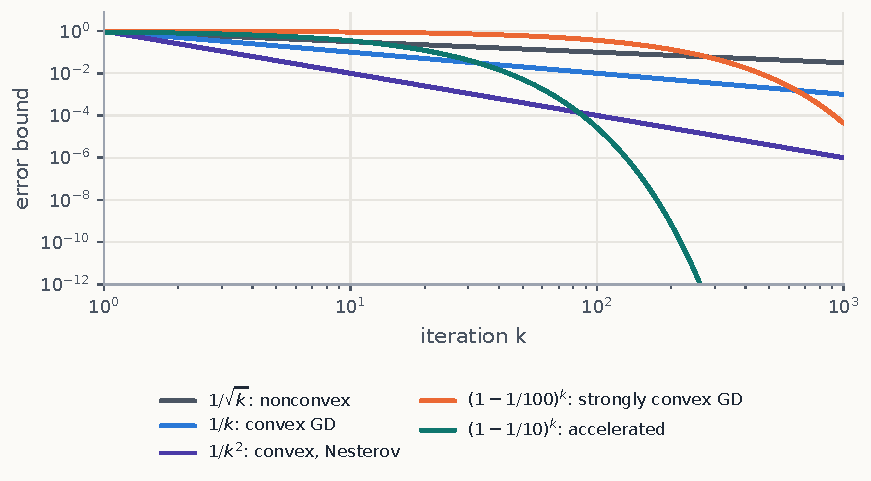
\includegraphics[width=\linewidth, height=0.62\textheight, keepaspectratio]{fig_rate_bounds}
    \end{column}
  \end{columns}
\end{frame}

% =====================================================================
%  7. When and why GD fails
% =====================================================================
\section{When and why GD fails}

\begin{frame}{The condition number in our own problems}
  \small
  $\kappa = \lmax/\lmin$ of the Hessian indicates how slowly GD may converge.
  \vspace{4pt}
  \begin{center}
  \begin{tabular}{@{}l c l@{}}
    \toprule
    Problem & $\kappa$ & Why \\
    \midrule
    M3: $x_1^2 + 4x_2^2$ & $4$ & curvatures $2$ and $8$ \\
    A1: line fit, raw weights & $28.7$ & columns $[\mathbf 1, x]$ point in similar directions \\
    A1: after centring $x$ & $1.04$ & centring removes the overlap \\
    A2: houses, raw features & $4.3\times10^{7}$ & sizes in the hundreds, bedrooms in units \\
    A2: after standardising & $14.4$ & same scale; size and bedrooms still move together \\
    Rosenbrock valley at $(1,1)$ & $2508$ & a narrow curved valley \\
    \bottomrule
  \end{tabular}
  \end{center}
  \footnotesize GD needs about $\kappa$ steps per digit of accuracy, so preprocessing that reduces $\kappa$ can speed up convergence.
\end{frame}

\begin{frame}{Why GD can fail}
  \centering
  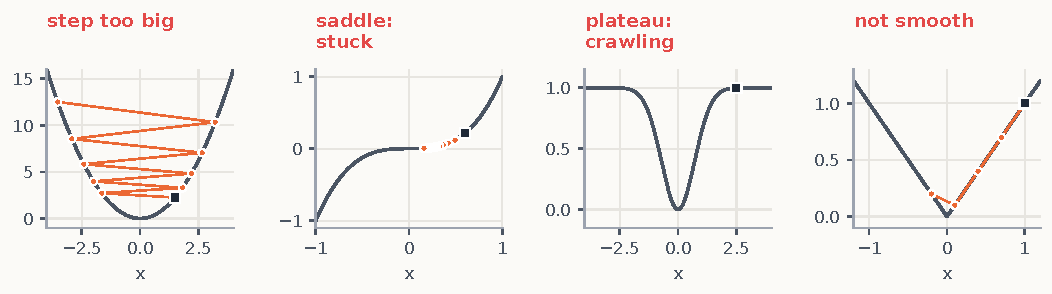
\includegraphics[width=\textwidth, height=0.36\textheight, keepaspectratio]{fig_failure_gallery}

  \raggedright\footnotesize
  \begin{columns}[T]
    \begin{column}{0.5\textwidth}
      \begin{itemize}
        \item \textbf{Step too big}: $\alpha > 2/f''$, each step overshoots further (Section 5).
        \item \textbf{Saddle}: on $x^3$ the slope $3x^2\to0$, so GD stalls at a point that is not a minimum. Saddles with some negative curvature are escaped almost surely from a random start~\cite{lee2016}.
      \end{itemize}
    \end{column}
    \begin{column}{0.48\textwidth}
      \begin{itemize}
        \item \textbf{Plateau}: the gradient is nearly zero, so GD barely moves.
        \item \textbf{Not smooth}: $|x|$ has no derivative at $0$; a fixed step keeps jumping across it.
              GD needs a smooth loss.
      \end{itemize}
    \end{column}
  \end{columns}
\end{frame}

\begin{frame}{Local minima and starting points}
  \begin{columns}[T]
    \begin{column}{0.52\textwidth}
      \centering
      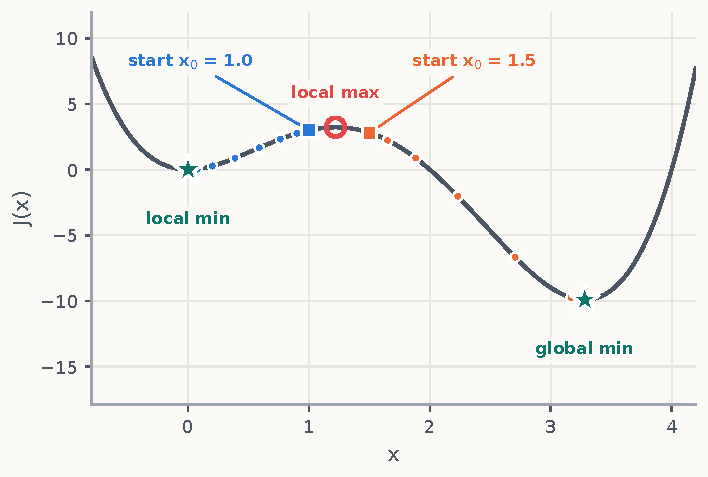
\includegraphics[width=\linewidth, height=0.6\textheight, keepaspectratio]{fig_local_minima}
    \end{column}
    \begin{column}{0.46\textwidth}
      \small
      $J(x) = x^4 - 6x^3 + 8x^2$ has two valleys with a hill at $x\approx1.22$.
      \begin{itemize}\footnotesize
        \item From $x_0 = 1.0$ GD rolls left into the \emph{local} minimum $x = 0$.
        \item From $x_0 = 1.5$ it rolls right into the \emph{global} minimum $x\approx3.28$.
      \end{itemize}
      GD may find \emph{a} minimum and miss \emph{the} best one.
      \begin{warnbox}[In practice]
        \footnotesize Try several starts and keep the best. The SSR of a line is convex: one minimum only.
      \end{warnbox}
    \end{column}
  \end{columns}
\end{frame}

% =====================================================================
%  8. Making it work better
% =====================================================================
\section{Making it work better}

\begin{frame}{Changing the learning rate as we go}
  \begin{columns}[T]
    \begin{column}{0.5\textwidth}
      \small
      \textbf{Schedule}~\cite{bottou2018}: start large, then shrink $\alpha$, e.g.
      \[
        \alpha_k = \frac{\alpha_0}{1 + \gamma k}.
      \]
      Smaller late steps help SGD settle (Section 9).

      \vspace{4pt}
      \textbf{Backtracking line search}~\cite{armijo1966}
      \par\footnotesize Try a step; if the loss did not drop enough, halve $\alpha$ and try again:
      \[
        \text{accept }\alpha\text{ if } J(\x - \alpha\g) \le J(\x) - c\,\alpha\norm{\g}^2 .
      \]
      This picks a safe step automatically, without knowing $f''$.
    \end{column}
    \begin{column}{0.48\textwidth}
      \begin{thmbox}[Rules of thumb]
        \small
        \begin{itemize}
          \item If the loss goes \emph{up}, $\alpha$ is too big: cut it by a factor of $10$.
          \item If the loss falls very slowly in a straight line, $\alpha$ is too small.
          \item Always keep a maximum number of steps.
          \item Scale the features first (Section 4): it widens the range of good $\alpha$.
        \end{itemize}
      \end{thmbox}
    \end{column}
  \end{columns}
\end{frame}

\begin{frame}{Heavy-ball momentum: give the point some mass}
  \small
  \textbf{Polyak's heavy ball}~\cite{polyak1964} adds a fraction $\beta$ of the last move:
  \[
    \x_{k+1} = \x_k - \alpha\nabla J(\x_k) + \beta\,(\x_k - \x_{k-1}),\qquad 0 \le \beta < 1 .
  \]
  Where it comes from: a ball of mass $m$ with friction $\gamma$ obeys $m\ddot\x + \gamma\dot\x = -\nabla J(\x)$.
  Replace the derivatives by finite differences with step $h$ and solve for $\x_{k+1}$:
  \[
    \x_{k+1} = \x_k - \underbrace{\tfrac{h^2}{m + \gamma h}}_{\alpha}\nabla J(\x_k) + \underbrace{\tfrac{m}{m + \gamma h}}_{\beta}(\x_k - \x_{k-1}).
  \]
  \begin{itemize}\footnotesize
    \item Along the valley the gradient keeps its sign, so the velocity \alert{builds up}.
          Across it the sign flips, so the moves \alert{cancel}: the zig-zag is damped.
    \item Plain GD is the massless ball, $\beta = 0$: the gradient-flow ODE of Section 3.
  \end{itemize}
\end{frame}

\begin{frame}{Why momentum is faster: $\kappa$ becomes $\sqrt\kappa$}
  \centering
  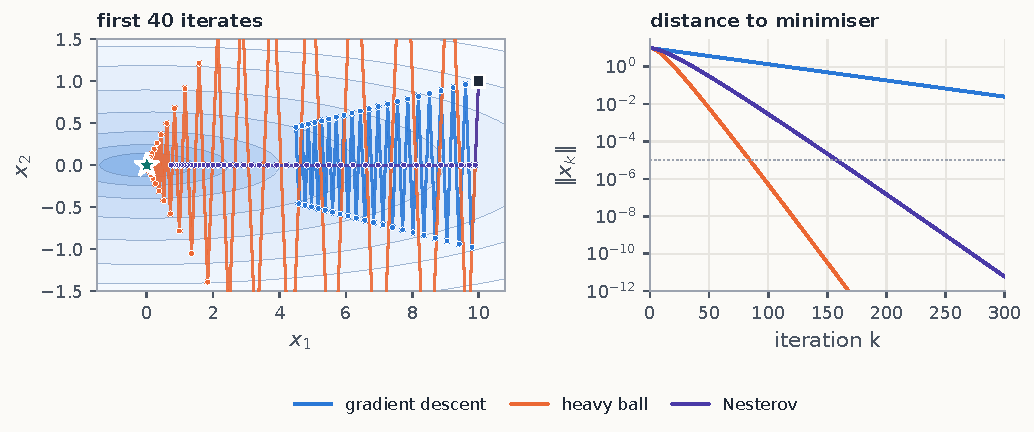
\includegraphics[width=0.86\textwidth, height=0.44\textheight, keepaspectratio]{fig_momentum}

  \raggedright\small
  \begin{columns}[T]
    \begin{column}{0.44\textwidth}
      On a quadratic, with the best $\alpha$ and $\beta$, the error factor per step is
      \[
        \rho_{\text{HB}} = \tfrac{\sqrt\kappa - 1}{\sqrt\kappa + 1}
        \quad\text{vs.}\quad
        \rho_{\text{GD}} = \tfrac{\kappa - 1}{\kappa + 1}.
      \]
    \end{column}
    \begin{column}{0.54\textwidth}
      \begin{itemize}\footnotesize
        \item $J = \tfrac12(x_1^2 + 100x_2^2)$, $\kappa = 100$: $0.818$ against $0.980$, about \alert{69} steps instead of
              \alert{691} for six digits. In the run: GD $691$, heavy ball $85$, Nesterov $158$.
        \item For nonquadratic losses, heavy ball can fail~\cite{lessard2016}. For illustrations, see~\cite{goh2017}.
      \end{itemize}
    \end{column}
  \end{columns}
\end{frame}

\begin{frame}{Nesterov: look ahead, then step}
  \small
  Take the gradient at a \textbf{look-ahead point}~\cite{nesterov1983}:
  \[
    \y_k = \x_k + \beta_k(\x_k - \x_{k-1}),\qquad \x_{k+1} = \y_k - \tfrac1L\nabla J(\y_k).
  \]
  This gives guarantees for \emph{every} smooth convex $J$, not just quadratics, and no first-order method can beat
  them by more than a constant~\cite{nesterov2018}:
  \begin{center}\footnotesize
  \begin{tabular}{@{}l c c c@{}}
    \toprule
    & GD & Nesterov & best possible \\
    \midrule
    convex, error after $k$ steps & $O(1/k)$ & $O(1/k^2)$ & $\Omega(1/k^2)$ \\
    strongly convex, steps to $\varepsilon$ & $O(\kappa\log\frac1\varepsilon)$ & $O(\sqrt\kappa\log\frac1\varepsilon)$ & $\Omega(\sqrt\kappa\log\frac1\varepsilon)$ \\
    $J$ goes down every step? & yes & no (it ripples) & \\
    \bottomrule
  \end{tabular}
  \end{center}
  \footnotesize Where GD needs $10^4$ steps, Nesterov needs about $200$. Its continuous-time limit is
  $\ddot\x + \frac3t\dot\x + \nabla J = 0$, a heavy ball whose friction fades~\cite{su2016}.
\end{frame}

\statement{CONDITIONING AND SPEED}{The condition number $\kappa$\\ controls the iteration count.}{GD needs about $\kappa$. Momentum and Nesterov need about $\sqrt\kappa$, and these rates are optimal for first-order methods.}

\begin{frame}{Adam: momentum plus a step size for every parameter}
  \begin{columns}[T]
    \begin{column}{0.5\textwidth}
      \small
      \textbf{Adam}~\cite{kingma2015}, all operations element-wise:
      \vspace{-4pt}
      \begin{align*}
        \mathbf m_k &= \beta_1\mathbf m_{k-1} + (1 - \beta_1)\g_k \\
        \mathbf v_k &= \beta_2\mathbf v_{k-1} + (1 - \beta_2)\g_k^{2} \\
        \x_{k+1} &= \x_k - \alpha\,\hat{\mathbf m}_k\big/\bigl(\sqrt{\hat{\mathbf v}_k} + \epsilon\bigr)
      \end{align*}
    \end{column}
    \begin{column}{0.48\textwidth}
      \begin{itemize}\footnotesize
        \item $\mathbf m$ is \alert{momentum}, as above.
        \item Dividing by $\sqrt{\mathbf v}$ gives each parameter its \alert{own learning rate}: automatic feature scaling (Section 4).
        \item The hats correct the start-up bias. Adam is a common deep learning optimiser.
      \end{itemize}
    \end{column}
  \end{columns}
  \centering
  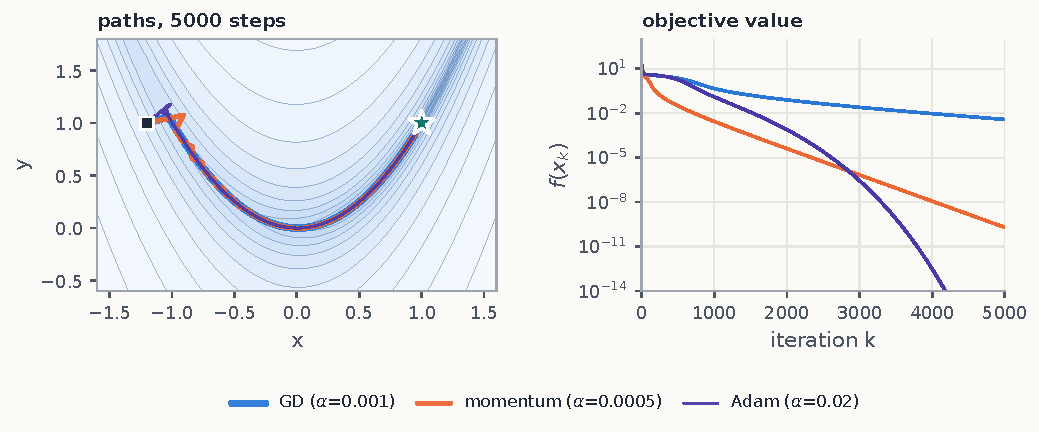
\includegraphics[width=0.86\textwidth, height=0.34\textheight, keepaspectratio]{fig_rosenbrock_race}

  \footnotesize Rosenbrock, $5000$ steps: GD is slow ($J \approx 4\times10^{-3}$), heavy ball reaches $2\times10^{-10}$, Adam reaches $(1, 1)$.
\end{frame}

% =====================================================================
%  9. At scale: SGD and modern practice
% =====================================================================
\section{At scale: SGD and modern practice}

\begin{frame}{When the data is huge: stochastic gradient descent}
  \small
  Plain (batch) GD uses \emph{every} data point to compute each gradient. With millions of points and parameters,
  one step is already expensive.
  \vspace{2pt}
  \begin{center}
  \begin{tabular}{@{}l l l@{}}
    \toprule
    Variant & data used per step & character \\
    \midrule
    batch GD & all $m$ points & smooth path, expensive steps \\
    stochastic GD (strict) & one random point & cheap, very noisy steps \\
    mini-batch GD (common practice) & a small random subset & cheap and fairly stable \\
    \bottomrule
  \end{tabular}
  \end{center}
  \begin{keybox}[Why use mini-batches~\cite{bottou2018}]
    \small Mini-batches give more stable estimates than one point, while keeping steps cheap.
    When \alert{new data} arrives, updates can continue from the current parameters.
  \end{keybox}
\end{frame}

\begin{frame}{What the noise looks like}
  \centering
  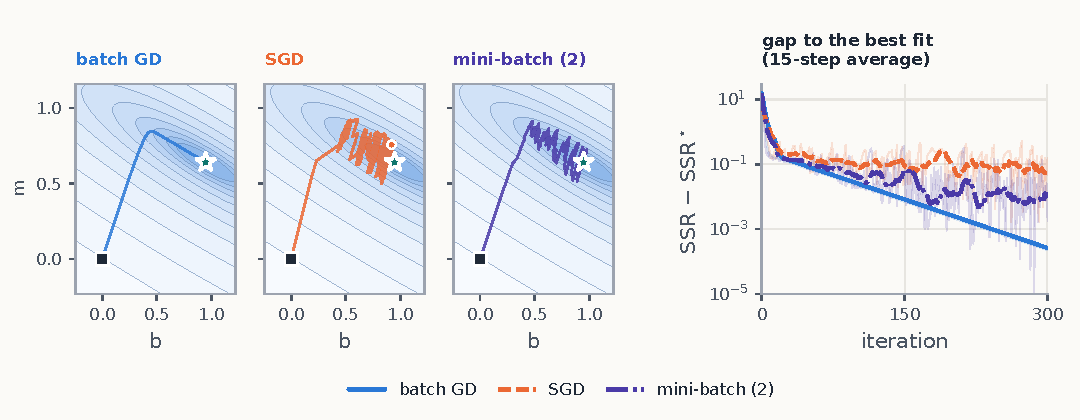
\includegraphics[width=\textwidth, height=0.55\textheight, keepaspectratio]{fig_sgd_paths}

  \raggedright\small
  \begin{itemize}
    \item One-point gradients are \emph{unbiased}: on average they equal the full gradient.
    \item Their noise does not vanish at the minimum, so with a fixed $\alpha$ SGD keeps jittering.
          Averaging $B$ points cuts the variance by $B$; a decaying $\alpha$ lets the path settle.
  \end{itemize}
\end{frame}

\begin{frame}{SGD's noise floor, and how a schedule removes it}
  \begin{columns}[T]
    \begin{column}{0.46\textwidth}
      \small
      One-sample gradients are right \emph{on average}, but at the minimum they are not zero:
      $\nabla J(w^\star) = 0$ while each $\nabla J_i(w^\star) \neq 0$.
      \begin{itemize}\footnotesize
        \item Constant $\alpha$: fast at first, then limited by a \alert{noise floor} that grows with $\alpha$.
        \item Decaying $\alpha_k$: the noise floor falls, at rate $O(1/k)$ for strongly convex $J$~\cite{bottou2018}.
      \end{itemize}
      \textbf{Robbins--Monro}~\cite{robbins1951}: SGD converges if
      \[
        \textstyle\sum_k \alpha_k = \infty, \qquad \sum_k \alpha_k^2 < \infty ,
      \]
      steps persist while their squared sizes remain summable.
    \end{column}
    \begin{column}{0.52\textwidth}
      \centering
      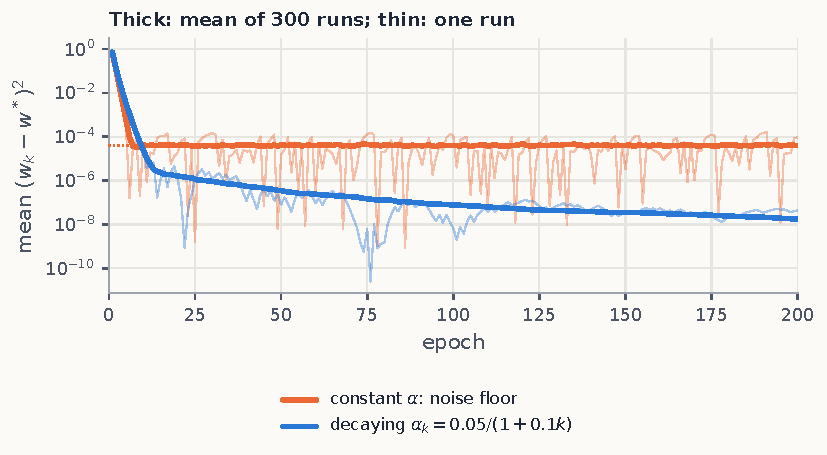
\includegraphics[width=\linewidth, height=0.6\textheight, keepaspectratio]{fig_sgd_noise}

      \footnotesize The sensor data of Problem A3, averaged over $300$ shuffled runs. After $200$ epochs: constant $\alpha$ sits near $4\times10^{-5}$, the schedule reaches $2\times10^{-8}$.
    \end{column}
  \end{columns}
\end{frame}

\begin{frame}{Where the gradient comes from: automatic differentiation}
  \begin{thmbox}[Cheap gradient principle~\cite{griewank2008}]
    Reverse-mode automatic differentiation computes the \emph{whole} gradient $\nabla J \in \R^n$ for a small constant
    times the cost of evaluating $J$ once, \alert{however large $n$ is}.
  \end{thmbox}
  \vspace{2pt}
  \centering\small
  \begin{tabular}{@{}l c c@{}}
    \toprule
    How we get $\nabla J$ & cost & accuracy \\
    \midrule
    by hand (as in Part B) & free once derived & exact \\
    finite differences, $\frac{J(\x + h\mathbf e_i) - J(\x)}{h}$ & $(n + 1)\times$ cost of $J$ & about $\sqrt{\epsilon_{\text{mach}}}$ \\
    reverse-mode AD (backpropagation) & a few times the cost of $J$ & machine precision \\
    \bottomrule
  \end{tabular}

  \raggedright\vspace{4pt}
  \footnotesize Backpropagation in neural networks \emph{is} reverse-mode AD. That, plus GD's $O(n)$ update, is why a
  model with $10^9$ parameters can be trained at all.
\end{frame}

\begin{frame}{Adaptive steps and stability}
  \begin{columns}[T]
    \begin{column}{0.48\textwidth}
      \textbf{Barzilai--Borwein: learn $\alpha$ from the last move}~\cite{barzilai1988}
      \small
      \[
        \alpha_k = \frac{\mathbf s\T\mathbf s}{\mathbf s\T\mathbf r},\qquad \mathbf s = \x_k - \x_{k-1},\ \ \mathbf r = \g_k - \g_{k-1}.
      \]
      \begin{itemize}\footnotesize
        \item $\mathbf r \approx H\mathbf s$, so $\alpha_k$ estimates $1/f''$ along the last step: Newton's step size, from gradients only.
        \item $J$ may briefly go \emph{up}, yet it is often faster than a fixed $\alpha$. Pair it with
              Armijo backtracking~\cite{armijo1966} for safety.
      \end{itemize}
    \end{column}
    \begin{column}{0.48\textwidth}
      \textbf{The edge of stability}~\cite{cohen2021}
      \begin{itemize}\small
        \item Theory says keep $\alpha < 2/L$.
        \item Yet when full-batch GD trains a neural network, the sharpness $\lmax$ \emph{rises} until it reaches
              $2/\alpha$, then hovers there while the loss keeps falling, unevenly.
        \item The analysis of Sections 5 and 6 does not explain this. It is an open research question.
      \end{itemize}
    \end{column}
  \end{columns}
\end{frame}

% =====================================================================
%  10. Summary
% =====================================================================
\nextsectionstop{11}
\section{Summary}

\begin{frame}{Gradient descent on two slides (1/2): the method}
  \centering\footnotesize
  \renewcommand{\arraystretch}{1.35}
  \begin{tabular}{@{}l l@{}}
    \toprule
    Idea & In one line \\
    \midrule
    update & $w_j \leftarrow w_j - \alpha\,\partial J/\partial w_j$ \quad (step size $=$ slope $\times$ learning rate) \\
    gradient & direction and size of the steepest slope; $-\nabla J$ is the steepest way down \\
    stop & step size $\approx0$, or maximum number of steps reached \\
    stability & converges only if $0 < \alpha < 2/f''$; best fixed $\alpha = 1/f''$ \\
    speed & linear order: error $\times\,|1-\alpha f''|$ per step; Newton is quadratic \\
    cost & $O(mn)$ per step, no matrix inversion: the reason ML uses it \\
    geometry & steps cross contours at right angles; stretched contours make it zig-zag \\
    failures & too-big $\alpha$, saddles, plateaus, non-smooth losses, local minima \\
    SGD & one point (or a mini-batch) per step: cheap and noisy; decay $\alpha$ to settle \\
    \bottomrule
  \end{tabular}
\end{frame}

\begin{frame}{Gradient descent on two slides (2/2): why it works}
  \centering\footnotesize
  \renewcommand{\arraystretch}{1.45}
  \begin{tabular}{@{}l l@{}}
    \toprule
    Idea & In one line \\
    \midrule
    ODE view & GD is forward Euler on $\dot\x = -\nabla J$; $\alpha < 2/\lmax$ is Euler's stability limit \\
    best step & on a quadratic $\alpha^\star = 2/(\lmin + \lmax)$, error factor $(\kappa - 1)/(\kappa + 1)$ \\
    guarantees & descent lemma: each step drops $J$ by $\norm{\g}^2/2L$; strongly convex gives $(1 - 1/\kappa)^k$ \\
    condition number & $\kappa = L/\mu$ means about $\kappa$ steps per digit; scaling features shrinks it \\
    momentum & heavy ball and Nesterov need about $\sqrt\kappa$, and no gradient method can do better \\
    SGD theory & a constant $\alpha$ leaves a noise floor; Robbins--Monro schedules remove it \\
    practice & Adam $=$ momentum $+$ per-parameter steps; backpropagation makes $\nabla J$ cheap \\
    \bottomrule
  \end{tabular}
\end{frame}

\statement{IN ONE SENTENCE}{Take a step downhill,\\ sized by the slope and the learning rate.}{Choose the learning rate carefully and check where the method converges.}


% ---------------- Part B ---------------------------------------------
\nextsectionlabel{B}
\nextsectionstop{10}
% =====================================================================
%  Part B -- Problem set overview
% =====================================================================
\section{Part B: problems and complete solutions}

\begin{frame}{Ten problems, each solved step by step}
  \small
  Each problem is followed \alert{right away} by a worked solution. Try it before turning the page.
  Every number in the solutions was checked by a script.

  \vspace{4pt}
  \begin{columns}[T]
    \begin{column}{0.49\textwidth}
      \textbf{Mathematical}
      \begin{itemize}\footnotesize
        \item[M1] Stationary points and local minima of a quartic
        \item[M2] Four learning rates on one parabola
        \item[M3] Two variables, contours and the zig-zag
        \item[M4] Scaling and shifting the loss
        \item[M5] GD against Newton
      \end{itemize}
    \end{column}
    \begin{column}{0.49\textwidth}
      \textbf{Real-life applications}
      \begin{itemize}\footnotesize
        \item[A1] Health: weight vs.\ height, the running example
        \item[A2] Real estate: house prices with two features
        \item[A3] Sensors: streaming data with SGD
        \item[A4] Engineering: the cheapest drink can
        \item[A5] Education: predicting pass or fail
      \end{itemize}
    \end{column}
  \end{columns}

  \vspace{4pt}
  \footnotesize\textcolor{mGrey}{Difficulty: $\star$ routine \quad $\star\star$ several steps \quad $\star\star\star$ deeper idea.}
\end{frame}

% =====================================================================
%  M1 -- Stationary points and local minima of a quartic
% =====================================================================
\subsection{M1: Stationary points of a quartic}
\setprob{M1}

\begin{frame}{\probtitle{M1}{Stationary points and two valleys}}
  \begin{probbox}[Problem M1 \hfill Mathematical \quad $\star\star$]
    Let $J(x) = x^4 - 6x^3 + 8x^2$.
    \begin{enumerate}[(a)]
      \item Find every stationary point of $J$.
      \item Use $J''$ to say which are minima and which are maxima. Which minimum is the lowest?
      \item Run three GD steps with $\alpha = 0.05$ from $x_0 = 1.0$, and again from $x_0 = 1.5$.
            Where does each run end up?
      \item How reliable is the result from a single GD run?
    \end{enumerate}
  \end{probbox}
  \footnotesize\textcolor{mGrey}{Practice: $J' = 0$, the second-derivative test, and the effect of the starting point.}
\end{frame}

\begin{frame}{\soltitle{M1}{1}{3}}
  \textbf{(a) Stationary points.} Set the slope to zero and factor out $2x$:
  \[
    J'(x) = 4x^3 - 18x^2 + 16x = 2x\,(2x^2 - 9x + 8) = 0 .
  \]
  So $x = 0$, or $x = \dfrac{9 \pm \sqrt{81 - 64}}{4} = \dfrac{9\pm\sqrt{17}}{4}$, which gives
  \[
    \ans{x = 0,\qquad x \approx 1.2192,\qquad x \approx 3.2808}
  \]
  \textbf{(b) Classify} with $J''(x) = 12x^2 - 36x + 16$:
  \begin{center}\small
  \begin{tabular}{@{}c c c l@{}}
    \toprule
    $x$ & $J''(x)$ & $J(x)$ & type \\
    \midrule
    $0$ & $16 > 0$ & $0$ & \textcolor{mTeal}{\textbf{local minimum}} \\
    $1.2192$ & $-10.05 < 0$ & $3.227$ & \textcolor{mOrange}{\textbf{maximum}} (the hill) \\
    $3.2808$ & $27.05 > 0$ & $-9.915$ & \textcolor{mTeal}{\textbf{global minimum}} \\
    \bottomrule
  \end{tabular}
  \end{center}
\end{frame}

\begin{frame}{\soltitle{M1}{2}{3}}
  \begin{columns}[T]
    \begin{column}{0.5\textwidth}
      \small
      \textbf{(c) GD with $\alpha = 0.05$}, $x_{k+1} = x_k - 0.05\,J'(x_k)$.

      \vspace{3pt}
      From $x_0 = 1.0$: $J'(1) = 4 - 18 + 16 = 2$, so $x_1 = 1 - 0.1 = 0.9$.
      \[
        1 \to 0.9 \to 0.763 \to 0.588 \to \ans{0}
      \]
      From $x_0 = 1.5$: $J'(1.5) = 13.5 - 40.5 + 24 = -3$, so $x_1 = 1.65$.
      \[
        1.5 \to 1.65 \to 1.882 \to 2.231 \to \ans{3.281}
      \]
      The two starts sit on opposite sides of the hill at $1.2192$.
    \end{column}
    \begin{column}{0.48\textwidth}
      \centering
      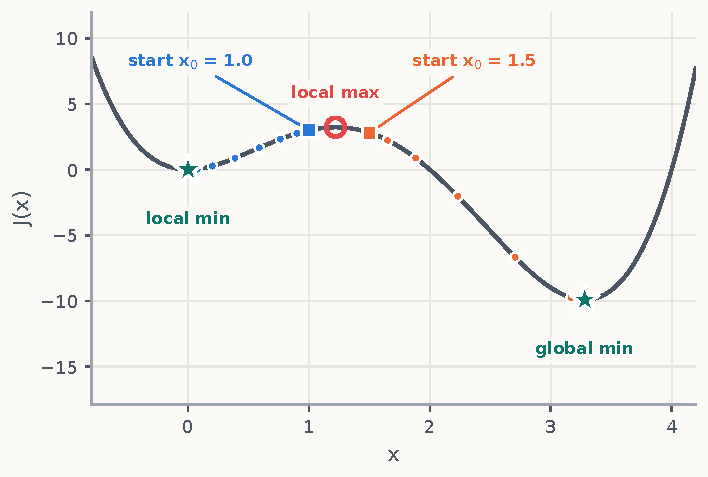
\includegraphics[width=\linewidth, height=0.62\textheight, keepaspectratio]{fig_local_minima}
    \end{column}
  \end{columns}
\end{frame}

\begin{frame}{\soltitle{M1}{3}{3}}
  \textbf{(d) What it means.}
  \begin{itemize}
    \item GD only follows the local slope. Start left of the hill and it settles at $x = 0$ with $J = 0$.
          Start right of it and it reaches $x \approx 3.28$ with $J \approx -9.92$.
    \item Both runs \emph{converged}: the step size went to zero in each. Convergence tells you that you reached
          a stationary point, not that you reached the best one.
    \item In practice, try several starting points and keep the lowest $J$.
  \end{itemize}
  \begin{keybox}[Answer]
    Stationary points $0,\ (9\pm\sqrt{17})/4$. The global minimum is $x^\star \approx 3.2808$, $J^\star \approx -9.915$.
    GD finds it only from starts to the right of the hill at $x \approx 1.2192$.
  \end{keybox}
\end{frame}

% =====================================================================
%  M2 -- Four learning rates on one parabola
% =====================================================================
\subsection{M2: Four learning rates}
\setprob{M2}

\begin{frame}{\probtitle{M2}{Four learning rates on one parabola}}
  \begin{probbox}[Problem M2 \hfill Mathematical \quad $\star$]
    Minimise $f(x) = (x-3)^2 + 2$ with GD from $x_0 = 0$.
    \begin{enumerate}[(a)]
      \item Write out $x_1, \dots, x_4$ for $\alpha = 0.1,\ 0.5,\ 0.9,\ 1.1$.
      \item Show that the error $e_k = x_k - 3$ obeys $e_{k+1} = (1 - 2\alpha)\,e_k$.
      \item Use (b) to explain each of the four behaviours.
      \item With $\alpha = 0.1$, how many steps cut the error by a factor of $10^6$?
    \end{enumerate}
  \end{probbox}
  \footnotesize\textcolor{mGrey}{Practice: running the update by hand, and the stability window for $\alpha$.}
\end{frame}

\begin{frame}{\soltitle{M2}{1}{3}}
  \textbf{(a) The iterates.} Here $f'(x) = 2(x - 3)$, so $x_{k+1} = x_k - 2\alpha(x_k - 3)$.
  \begin{center}\small
  \begin{tabular}{@{}c c c c c l@{}}
    \toprule
    $\alpha$ & $x_1$ & $x_2$ & $x_3$ & $x_4$ & behaviour \\
    \midrule
    $0.1$ & $0.6$ & $1.08$ & $1.464$ & $1.7712$ & creeps up from one side \\
    $0.5$ & $3$ & $3$ & $3$ & $3$ & exact in \emph{one} step \\
    $0.9$ & $5.4$ & $1.08$ & $4.536$ & $1.7712$ & jumps across, closes in \\
    $1.1$ & $6.6$ & $-1.32$ & $8.184$ & $-3.2208$ & \textcolor{mRed}{\textbf{diverges}} \\
    \bottomrule
  \end{tabular}
  \end{center}
  For example, with $\alpha = 0.1$: $x_1 = 0 - 0.2\,(0 - 3) = 0.6$, then $x_2 = 0.6 - 0.2\,(0.6 - 3) = 1.08$.

  \vspace{3pt}
  \footnotesize\textcolor{mGrey}{The figure in Section 5 shows the same four regimes, drawn with $\alpha = 1.05$ for the last one.}
\end{frame}

\begin{frame}{\soltitle{M2}{2}{3}}
  \textbf{(b) The error recursion.} Subtract $3$ from both sides of the update:
  \[
    x_{k+1} - 3 = (x_k - 3) - 2\alpha(x_k - 3)
    \quad\Longrightarrow\quad \ans{e_{k+1} = (1 - 2\alpha)\,e_k},
    \qquad e_k = (1-2\alpha)^k e_0 .
  \]
  \textbf{(c) Reading the factor} $\rho = 1 - 2\alpha$, with $e_0 = -3$:
  \begin{itemize}\small
    \item $\alpha = 0.1$: $\rho = 0.8$. Same sign every step, shrinking by $20\%$: a slow, one-sided approach.
    \item $\alpha = 0.5$: $\rho = 0$. The error vanishes after one step.
    \item $\alpha = 0.9$: $\rho = -0.8$. The sign flips each step but $|\rho| < 1$, so it still converges.
    \item $\alpha = 1.1$: $\rho = -1.2$. The sign flips and $|e_k|$ grows by $20\%$ each step.
  \end{itemize}
  So GD converges exactly when $|1 - 2\alpha| < 1$, that is $\ans{0 < \alpha < 1}$, which matches $2/f'' = 2/2$.
\end{frame}

\begin{frame}{\soltitle{M2}{3}{3}}
  \textbf{(d) Counting steps for $\alpha = 0.1$.} We need $|e_k/e_0| = 0.8^k \le 10^{-6}$:
  \[
    k \ge \frac{\ln 10^{6}}{\ln(1/0.8)} = \frac{13.816}{0.2231} = 61.9
    \quad\Longrightarrow\quad \ans{k = 62}
  \]
  Check: $0.8^{61} = 1.23\times10^{-6}$ is not enough, while $0.8^{62} = 9.8\times10^{-7}$ is.
  \begin{keybox}[Take-away]
    With the function and start fixed, the outcome depends on $\alpha$.
    The best fixed step is $\alpha = 1/f'' = 0.5$; anything past $2/f'' = 1$ diverges.
  \end{keybox}
\end{frame}

% =====================================================================
%  M3 -- Two variables, contours and the zig-zag
% =====================================================================
\subsection{M3: Two variables and the zig-zag}
\setprob{M3}

\begin{frame}{\probtitle{M3}{Two variables, contours and the zig-zag}}
  \begin{probbox}[Problem M3 \hfill Mathematical \quad $\star\star$]
    Let $J(x_1, x_2) = x_1^2 + 4x_2^2$ and start from $\x_0 = (2, 1)$.
    \begin{enumerate}[(a)]
      \item Find $\nabla J$ and take two GD steps with $\alpha = 0.1$. Does $J$ go down?
      \item What is the largest $\alpha$ for which GD still converges? Take two steps with $\alpha = 0.2$.
      \item Repeat (a) on the round bowl $x_1^2 + x_2^2$. Compare the two paths.
    \end{enumerate}
  \end{probbox}
  \footnotesize\textcolor{mGrey}{Practice: the update with several parameters, and how the shape of the contours changes GD.}
\end{frame}

\begin{frame}{\soltitle{M3}{1}{3}}
  \textbf{(a) Two steps with $\alpha = 0.1$.} $\nabla J = (2x_1,\ 8x_2)$, so each coordinate has its own factor:
  \[
    x_1 \leftarrow (1 - 2\alpha)\,x_1 = 0.8\,x_1, \qquad x_2 \leftarrow (1 - 8\alpha)\,x_2 = 0.2\,x_2 .
  \]
  \begin{center}\small
  \begin{tabular}{@{}c c c c@{}}
    \toprule
    step & $\x_k$ & $\nabla J(\x_k)$ & $J(\x_k)$ \\
    \midrule
    0 & $(2,\ 1)$ & $(4,\ 8)$ & $8$ \\
    1 & $(1.6,\ 0.2)$ & $(3.2,\ 1.6)$ & $2.72$ \\
    2 & $\ans{(1.28,\ 0.04)}$ & $(2.56,\ 0.32)$ & $1.6448$ \\
    \bottomrule
  \end{tabular}
  \end{center}
  $J$ falls from $8$ to $1.64$. The steep $x_2$ direction is almost done after two steps, but $x_1$ has only
  lost $36\%$: the flat direction is the slow one.
\end{frame}

\begin{frame}{\soltitle{M3}{2}{3}}
  \begin{columns}[T]
    \begin{column}{0.52\textwidth}
      \small
      \textbf{(b) Largest stable $\alpha$.} Both factors must satisfy $|1 - 2\alpha| < 1$ and $|1 - 8\alpha| < 1$.
      The steep direction is stricter:
      \[
        0 < \alpha < \tfrac{2}{8} = \ans{0.25}
      \]
      With $\alpha = 0.2$ the factors are $0.6$ and $-0.6$:
      \[
        (2, 1)\to(1.2,\ -0.6)\to(0.72,\ 0.36)
      \]
      $x_2$ flips sign every step. That is the \alert{zig-zag} across the valley. It still converges, since $0.6 < 1$.
    \end{column}
    \begin{column}{0.46\textwidth}
      \centering
      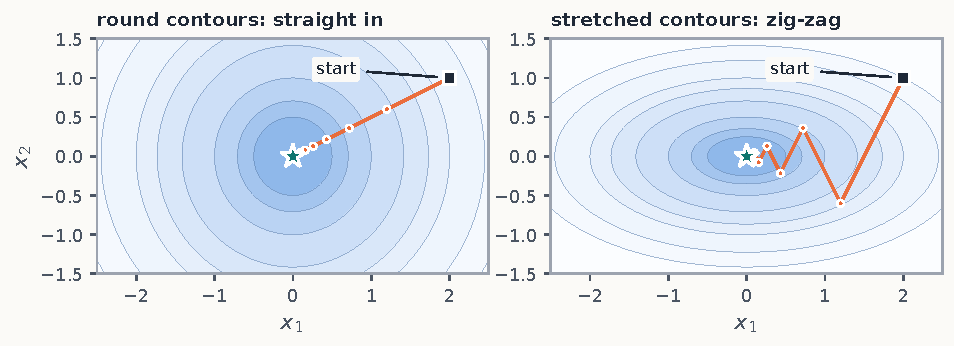
\includegraphics[width=\linewidth, height=0.6\textheight, keepaspectratio]{fig_zigzag_scaling}
    \end{column}
  \end{columns}
\end{frame}

\begin{frame}{\soltitle{M3}{3}{3}}
  \textbf{(c) The round bowl $x_1^2 + x_2^2$.} Now $\nabla J = (2x_1, 2x_2)$, and with $\alpha = 0.1$ both factors are $0.8$:
  \[
    (2, 1) \to (1.6,\ 0.8) \to \ans{(1.28,\ 0.64)},\qquad J:\ 5 \to 3.2 \to 2.048 .
  \]
  Every point is a multiple of $(2,1)$: the path is a \alert{straight line} into the minimum, because $-\nabla J$ points
  right at it.
  \begin{keybox}[Take-away]
    On the round bowl any $\alpha < 1$ works and $\alpha = 0.5$ finishes in one step.
    On the stretched bowl the steep direction caps $\alpha$ at $0.25$, and the flat direction converges slowly.
    Equal curvatures speed up GD.
  \end{keybox}
\end{frame}

% =====================================================================
%  M4 -- Scaling and shifting the loss
% =====================================================================
\subsection{M4: Scaling and shifting the loss}
\setprob{M4}

\begin{frame}{\probtitle{M4}{SSR or MSE? Scaling and shifting the loss}}
  \begin{probbox}[Problem M4 \hfill Mathematical \quad $\star\star$]
    Use the clinic data $x = (0.5, 2.3, 2.9)$, $y = (1.4, 1.9, 3.2)$ with the slope fixed at $0.64$.
    Compare two losses for the intercept $b$:
    \[
      \SSR(b) = \sum_{i=1}^{3}(y_i - b - 0.64x_i)^2, \qquad J(b) = \frac{1}{2m}\,\SSR(b),\ m = 3 .
    \]
    \begin{enumerate}[(a)]
      \item Find both gradients at $b = 0$ and the first GD step with $\alpha = 0.1$.
      \item Do the two losses have the same minimiser? Find it.
      \item What changes if we add the constant $2$ to the loss?
    \end{enumerate}
  \end{probbox}
\end{frame}

\begin{frame}{\soltitle{M4}{1}{2}}
  \textbf{(a) Gradients at $b = 0$.} Write $r_i = y_i - 0.64x_i = (1.08,\ 0.428,\ 1.344)$, so $\sum r_i = 2.852$.
  \[
    \frac{d\,\SSR}{db} = -2\sum_i (r_i - b) = -2(2.852) = -5.704,
    \qquad
    \frac{dJ}{db} = \frac{1}{6}\,\frac{d\,\SSR}{db} = -0.9507 .
  \]
  First step with $\alpha = 0.1$:
  \[
    \SSR:\ b_1 = 0 + 0.5704 = \ans{0.5704}, \qquad J:\ b_1 = 0 + 0.09507 = \ans{0.0951}
  \]
  Same direction, but the MSE step is $2m = 6$ times smaller. Dividing the loss by $6$ is the same as dividing
  $\alpha$ by $6$: $\alpha = 0.6$ on $J$ takes exactly the SSR steps.
\end{frame}

\begin{frame}{\soltitle{M4}{2}{2}}
  \textbf{(b) Same minimiser.} Setting either derivative to zero gives the same equation, $\sum_i (r_i - b) = 0$:
  \[
    b^\star = \frac{1}{3}\sum_i r_i = \frac{2.852}{3} = \ans{0.9507}
  \]
  Scaling a loss by a positive number cannot move its lowest point; both GD runs end at $0.950667$.

  \textbf{(c) Adding $2$.} $\SSR(0)$ goes from $3.156$ to $5.156$, but the derivative of a constant is zero, so the
  gradient, every step and the minimiser are \alert{unchanged}.
  \begin{keybox}[Take-away]
    \small GD uses the slope: shifting leaves updates unchanged; scaling rescales $\alpha$.
    In $\tfrac{1}{2m}$, the $\tfrac12$ cancels the $2$ from the square and $\tfrac1m$ makes $\alpha$ independent of the data size.
  \end{keybox}
\end{frame}

% =====================================================================
%  M5 -- GD against Newton
% =====================================================================
\subsection{M5: GD against Newton}
\setprob{M5}

\begin{frame}{\probtitle{M5}{GD against Newton}}
  \begin{probbox}[Problem M5 \hfill Mathematical \quad $\star\star\star$]
    \begin{enumerate}[(a)]
      \item Apply one Newton step, $x_{k+1} = x_k - f'(x_k)/f''(x_k)$, to $f(x) = (x-3)^2$ from $x_0 = 0$.
            How many GD steps with $\alpha = 0.1$ reach the same accuracy (error cut by $10^6$)?
      \item Now take $J(x) = x^4 - 6x^3 + 8x^2$ from Problem M1 and start at $x_0 = 1.4$.
            Run Newton and GD ($\alpha = 0.05$). Where does each one go?
      \item Which method would you trust here, and why?
    \end{enumerate}
  \end{probbox}
  \footnotesize\textcolor{mGrey}{Practice: comparing GD and Newton with numerical examples.}
\end{frame}

\begin{frame}{\soltitle{M5}{1}{3}}
  \begin{columns}[T]
    \begin{column}{0.52\textwidth}
      \small
      \textbf{(a) Newton on a parabola.} $f'(0) = -6$ and $f'' = 2$:
      \[
        x_1 = 0 - \frac{-6}{2} = \ans{3}
      \]
      Newton reaches the minimum. Newton fits a parabola to $f$, and here $f$ \emph{is} a parabola.

      \vspace{3pt}
      GD with $\alpha = 0.1$ cuts the error by $0.8$ per step, so it needs $\ans{62}$ steps
      (Problem M2). Newton's step is $\alpha = 1/f''$, the best possible fixed rate.
    \end{column}
    \begin{column}{0.46\textwidth}
      \centering
      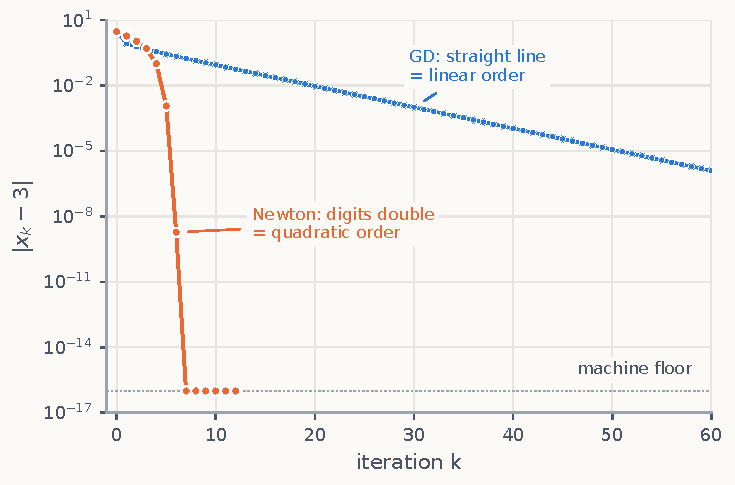
\includegraphics[width=\linewidth, height=0.6\textheight, keepaspectratio]{fig_gd_vs_newton}
    \end{column}
  \end{columns}
\end{frame}

\begin{frame}{\soltitle{M5}{2}{3}}
  \textbf{(b) Start at $x_0 = 1.4$ on the quartic.} Here $J'(1.4) = -1.904$ and $J''(1.4) = -10.88 < 0$:
  the curve bends \emph{down}.

  \vspace{3pt}
  \textbf{Newton:} $x_1 = 1.4 - \dfrac{-1.904}{-10.88} = 1.4 - 0.175 = 1.225$, then
  \[
    1.4 \to 1.225 \to 1.21923 \to \ans{1.21922} \quad\text{the \textcolor{mRed}{maximum}, } J = 3.227 .
  \]
  \textbf{GD:} $x_1 = 1.4 - 0.05(-1.904) = 1.4952$, then
  \[
    1.4 \to 1.4952 \to 1.6426 \to 1.8704 \to\cdots\to \ans{3.2808}\quad\text{the global minimum, } J = -9.915 .
  \]
  Newton converged quickly to a maximum.
\end{frame}

\begin{frame}{\soltitle{M5}{3}{3}}
  \textbf{(c) Why.} Newton solves $J'(x) = 0$. It cannot tell a minimum from a maximum, and where $J'' < 0$
  its step points \emph{uphill}. GD steps along $-J'$, which always points downhill, so $J$ decreases for any
  small enough $\alpha$.
  \begin{center}\small
  \begin{tabular}{@{}l c c@{}}
    \toprule
    from $x_0 = 1.4$ & Newton & GD, $\alpha = 0.05$ \\
    \midrule
    limit & $1.2192$ (maximum) & $3.2808$ (minimum) \\
    speed near the limit & quadratic & linear \\
    \bottomrule
  \end{tabular}
  \end{center}
  \begin{keybox}[Take-away]
    Trust GD far from the answer, and Newton close to a minimum where $J'' > 0$.
    Levenberg--Marquardt~\cite{nocedal2006} uses both gradients and curvature.
  \end{keybox}
\end{frame}

% =====================================================================
%  A1 -- Health: weight vs height, the running example
% =====================================================================
\subsection{A1: Health, weight against height}
\setprob{A1}

\begin{frame}{\probtitle{A1}{Health: predicting height from weight}}
  \begin{probbox}[Problem A1 \hfill Application \quad $\star$]
    A clinic records weight $x$ and height $y$ for three people: $x = (0.5,\ 2.3,\ 2.9)$, $y = (1.4,\ 1.9,\ 3.2)$.
    Fit $\hat y = b + m x$ by minimising $\SSR(b, m)$.
    \begin{enumerate}[(a)]
      \item Fix $m = 0.64$. Run three GD steps on $b$ from $b_0 = 0$ with $\alpha = 0.1$.
            When does the condition ``stop when $|\text{step}| < 0.001$'' hold?
      \item Now move both: start at $(b, m) = (0, 1)$ with $\alpha = 0.01$ and take two steps.
      \item Solve the least-squares equations by hand and compare with where GD ends.
    \end{enumerate}
  \end{probbox}
  \footnotesize\textcolor{mGrey}{Practice: steps (i)--(vi), worked by hand.}
\end{frame}

\begin{frame}{\soltitle{A1}{1}{3}}
  \textbf{(a) Intercept only.} $\dfrac{d\,\SSR}{db} = -2\sum_i(y_i - b - 0.64x_i)$, step $=$ slope $\times\,0.1$, $b \leftarrow b - \text{step}$.
  \begin{center}\small
  \begin{tabular}{@{}c c c c@{}}
    \toprule
    step & slope $d\SSR/db$ & step size & new $b$ \\
    \midrule
    1 & $-5.704$ & $-0.5704$ & $0.5704$ \\
    2 & $-2.2816$ & $-0.22816$ & $0.79856$ \\
    3 & $-0.91264$ & $-0.091264$ & $0.889824$ \\
    \bottomrule
  \end{tabular}
  \end{center}
  Each step is $0.4$ times the one before, so it takes \ans{8} updates for the step to drop below $0.001$
  (last step $0.00093$). GD stops at $b = 0.9500$, just short of $b^\star = 0.9507$.
\end{frame}

\begin{frame}{\soltitle{A1}{2}{3}}
  \textbf{(b) Both parameters.} The residuals at $(b, m) = (0, 1)$ are $y_i - x_i = (0.9,\ -0.4,\ 0.3)$:
  \[
    \frac{\partial\SSR}{\partial b} = -2(0.9 - 0.4 + 0.3) = -1.6,\qquad
    \frac{\partial\SSR}{\partial m} = -2(0.45 - 0.92 + 0.87) = -0.8 .
  \]
  Both move \emph{at the same time}, with $\alpha = 0.01$:
  \[
    (b, m)_1 = (0 + 0.016,\ 1 + 0.008) = \ans{(0.016,\ 1.008)}
  \]
  At the new point the gradient is $(-1.4128,\ -0.3944)$, so
  \[
    (b, m)_2 = \ans{(0.030128,\ 1.01194)}
  \]
  After \alert{808} updates both steps are below $10^{-6}$ and $(b, m) = (0.94863,\ 0.64106)$.
\end{frame}

\begin{frame}{\soltitle{A1}{3}{3}}
  \begin{columns}[T]
    \begin{column}{0.54\textwidth}
      \small
      \textbf{(c) Least squares by hand.} With $n = 3$, $\sum x = 5.7$, $\sum y = 6.5$, $\sum x^2 = 13.95$, $\sum xy = 14.35$:
      \[
        m = \frac{n\sum xy - \sum x\sum y}{n\sum x^2 - (\sum x)^2} = \frac{6.00}{9.36} = \ans{0.641026}
      \]
      \[
        b = \frac{\sum y - m\sum x}{n} = \ans{0.948718}
      \]
      GD matched both to within $10^{-4}$. Here a closed form is easy; GD uses the gradient instead.
    \end{column}
    \begin{column}{0.44\textwidth}
      \centering
      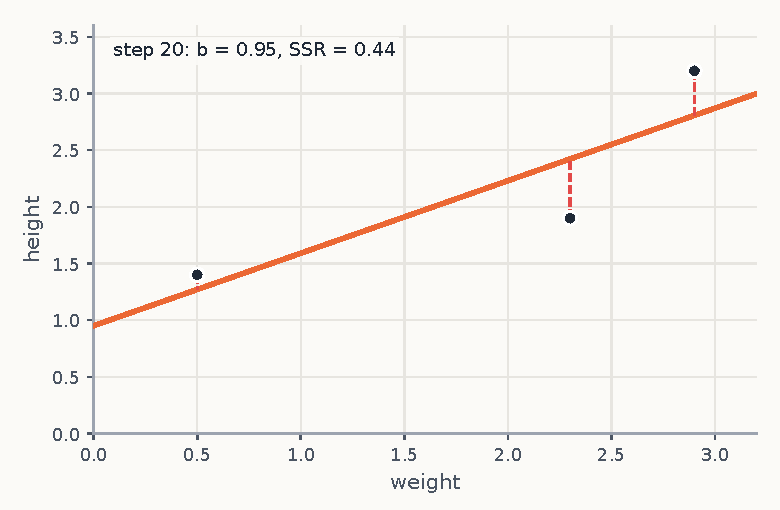
\includegraphics[width=\linewidth, height=0.58\textheight, keepaspectratio]{fig_line_frame_5}
    \end{column}
  \end{columns}
\end{frame}

% =====================================================================
%  A2 -- Real estate: house prices with two features
% =====================================================================
\subsection{A2: Real estate, house prices}
\setprob{A2}

\begin{frame}{\probtitle{A2}{Real estate: pricing houses with two features}}
  \begin{probbox}[Problem A2 \hfill Application \quad $\star\star\star$]
    Four flats in Dhaka:
    \begin{center}\small
    \begin{tabular}{@{}l c c c c@{}}
      size (sq ft) & 800 & 1000 & 1200 & 1500 \\
      bedrooms & 2 & 2 & 3 & 3 \\
      price (lakh Tk) & 40 & 50 & 60 & 70 \\
    \end{tabular}
    \end{center}
    Fit $\hat y = w_0 + w_1\,\text{size} + w_2\,\text{beds}$ with $J(\w) = \frac{1}{2m}\sum_i(\hat y_i - y_i)^2$.
    \begin{enumerate}[(a)]
      \item Find $\nabla J$ at $\w = \mathbf 0$ on the raw data. Why is plain GD slow here?
      \item Standardise both features and run GD with $\alpha = 0.1$. Map the weights back to original units.
      \item Check with the normal equation, then price a 1100 sq ft, 2-bedroom flat.
    \end{enumerate}
  \end{probbox}
\end{frame}

\begin{frame}{\soltitle{A2}{1}{3}}
  \textbf{(a) The raw gradient.} At $\w = \mathbf 0$, $\nabla J = \tfrac1m\bX\T(\bX\w - \vy) = -\tfrac1m\bX\T\vy$:
  \[
    \nabla J(\mathbf 0) = \bigl(-55,\ \ -64\,750,\ \ -142.5\bigr).
  \]
  The size component is hundreds of times bigger than the others, because sizes are in the hundreds.
  \begin{itemize}\small
    \item Stability needs $\alpha < 2/\lambda_{\max}$, where $\lambda_{\max} = 1.33\times10^{6}$ is the largest curvature.
          So $\alpha < \ans{1.5\times10^{-6}}$.
    \item With such a tiny $\alpha$, the step for $w_0$ is about $10^{-6}\times55$: the intercept barely moves.
  \end{itemize}
  This is the stretched-contour zig-zag of Section 4, with very unequal scales.
\end{frame}

\begin{frame}{\soltitle{A2}{2}{3}}
  \textbf{(b) Standardise}, $z = (\text{value} - \text{mean})/\text{std}$:
  size mean $1125$, std $258.60$; beds mean $2.5$, std $0.5$.

  \vspace{3pt}
  Now every feature has a similar scale, and GD with $\alpha = 0.1$ converges in $1391$ steps
  (until $\norm{\nabla J} < 10^{-8}$) to
  \[
    \hat y = 55 + 9.946\,z_{\text{size}} + 1.346\,z_{\text{beds}} .
  \]
  \textbf{Back to original units:} divide each weight by its std, then fix the intercept.
  \[
    w_1 = \tfrac{9.946}{258.60} = 0.03846,\qquad w_2 = \tfrac{1.346}{0.5} = 2.692,
  \]
  \[
    w_0 = 55 - 0.03846(1125) - 2.692(2.5) = 5.000 .
  \]
\end{frame}

\begin{frame}{\soltitle{A2}{3}{3}}
  \textbf{(c) Normal equation check.} Solving $\bX\T\bX\,\w = \bX\T\vy$ directly gives
  \[
    \w = (5,\ 0.038462,\ 2.692308),
  \]
  the same as GD to within $10^{-7}$. So the model is
  \[
    \text{price} \approx 5 + 0.0385\times\text{size} + 2.69\times\text{beds}\quad\text{(lakh Tk)}.
  \]
  For 1100 sq ft and 2 bedrooms: $5 + 42.31 + 5.38 = \ans{52.69\text{ lakh Tk}}$.
  \begin{keybox}[Take-away]
    A large feature scale slows raw GD; standardising the same data speeds convergence.
    Each extra square foot adds about Tk 3,850, and each extra bedroom about Tk 2.7 lakh.
  \end{keybox}
\end{frame}

% =====================================================================
%  A3 -- Sensors: streaming data with SGD
% =====================================================================
\subsection{A3: Sensors, streaming data with SGD}
\setprob{A3}

\begin{frame}{\probtitle{A3}{Sensors: calibrating with streaming data}}
  \begin{probbox}[Problem A3 \hfill Application \quad $\star\star$]
    A sensor gives readings $y$ for known inputs $x$: $(1,\ 2.1)$, $(2,\ 3.9)$, $(3,\ 6.2)$.
    Calibrate $\hat y = w x$ with the per-sample loss $\tfrac12(wx_i - y_i)^2$, $w_0 = 0$, $\alpha = 0.05$.
    \begin{enumerate}[(a)]
      \item Run one SGD epoch (samples in order 1, 2, 3).
      \item Compare with one batch GD step, and with mini-batches $\{1,2\}$ then $\{3\}$.
      \item Find the exact $w^\star$. After 50 epochs, compare a constant $\alpha$ with $\alpha_k = 0.05/(1 + 0.1k)$.
      \item A new reading $(4,\ 8.1)$ arrives. Update the model without starting again.
    \end{enumerate}
  \end{probbox}
\end{frame}

\begin{frame}{\soltitle{A3}{1}{3}}
  \textbf{(a) One SGD epoch.} For one sample the gradient is $(wx_i - y_i)\,x_i$, and $w \leftarrow w - 0.05\times$ gradient.
  \begin{center}\small
  \begin{tabular}{@{}c c c c@{}}
    \toprule
    sample & $(x_i, y_i)$ & gradient & new $w$ \\
    \midrule
    1 & $(1,\ 2.1)$ & $(0 - 2.1)(1) = -2.1$ & $0.105$ \\
    2 & $(2,\ 3.9)$ & $(0.21 - 3.9)(2) = -7.38$ & $0.474$ \\
    3 & $(3,\ 6.2)$ & $(1.422 - 6.2)(3) = -14.334$ & $\ans{1.1907}$ \\
    \bottomrule
  \end{tabular}
  \end{center}
  SGD makes one cheap update per reading as data arrives.
\end{frame}

\begin{frame}{\soltitle{A3}{2}{3}}
  \textbf{(b) Batch and mini-batch.} Each uses the \emph{mean} gradient of its samples.
  \begin{itemize}\small
    \item \textbf{Batch:} mean gradient at $w = 0$ is $-(2.1 + 7.8 + 18.6)/3 = -9.5$, so $w_1 = \ans{0.475}$.
          After three batch steps $w = 1.118$, still below the SGD epoch's $1.191$.
    \item \textbf{Mini-batch $\{1,2\}$:} mean gradient $-(2.1 + 7.8)/2 = -4.95$, so $w = 0.2475$.
          Then $\{3\}$: $(0.7425 - 6.2)(3) = -16.37$, so $w = \ans{1.0661}$.
  \end{itemize}
  \textbf{(c) Exact answer.} Setting $\sum_i (wx_i - y_i)x_i = 0$:
  \[
    w^\star = \frac{\sum x_iy_i}{\sum x_i^2} = \frac{28.5}{14} = \ans{2.0357}
  \]
  After 50 epochs: constant $\alpha$ gives $w = 2.0459$ (off by $0.010$);
  the decaying schedule gives $w = 2.0374$ (off by $0.0016$), six times closer.
\end{frame}

\begin{frame}{\soltitle{A3}{3}{3}}
  \textbf{Why the constant rate stalls.} Each sample pulls $w$ towards its own best fit
  ($2.1$, $1.95$, $2.07$). With a fixed $\alpha$ the last pull always wins a little, so SGD settles at a slightly
  biased point. A shrinking $\alpha$ makes those pulls fade.

  \vspace{4pt}
  \textbf{(d) New reading $(4,\ 8.1)$.} Continue from the constant-rate model $w = 2.0459$:
  \[
    \text{gradient} = (2.0459\times4 - 8.1)(4) = 0.334,\qquad
    w \leftarrow 2.0459 - 0.05(0.334) = \ans{2.0292}
  \]
  One update incorporates the new reading.
  \begin{keybox}[Take-away]
    SGD trades exact gradients for cheap updates. A decaying learning rate helps it settle.
  \end{keybox}
\end{frame}

% =====================================================================
%  A4 -- Engineering: the cheapest drink can
% =====================================================================
\subsection{A4: Engineering, the cheapest can}
\setprob{A4}

\begin{frame}{\probtitle{A4}{Engineering: the cheapest drink can}}
  \begin{probbox}[Problem A4 \hfill Application \quad $\star\star$]
    A factory makes cylindrical cans holding $V = 500\text{ cm}^3$. Less metal means lower cost, so minimise the surface area
    \[
      A(r) = 2\pi r^2 + 2\pi r h,\qquad h = \frac{V}{\pi r^2}
      \quad\Longrightarrow\quad A(r) = 2\pi r^2 + \frac{1000}{r}.
    \]
    \begin{enumerate}[(a)]
      \item Find $r^\star$, $h^\star$ and $A^\star$ exactly.
      \item Run GD from $r_0 = 2$ cm with $\alpha = 0.01$. How many steps until $|A'| < 10^{-6}$?
      \item What is the largest stable $\alpha$ near $r^\star$? Try $\alpha = 0.06$ from $r_0 = 4$.
    \end{enumerate}
  \end{probbox}
\end{frame}

\begin{frame}{\soltitle{A4}{1}{3}}
  \begin{columns}[T]
    \begin{column}{0.52\textwidth}
      \small
      \textbf{(a) Exact optimum.}
      \[
        A'(r) = 4\pi r - \frac{1000}{r^2} = 0
        \;\Longrightarrow\; r^\star = \Bigl(\frac{250}{\pi}\Bigr)^{1/3}
      \]
      \[
        \ans{r^\star = 4.301\text{ cm},\quad h^\star = 8.603\text{ cm} = 2r^\star}
      \]
      $A^\star = 348.73\text{ cm}^2$. Since $A''(r) = 4\pi + 2000/r^3 > 0$ for all $r > 0$, this is the only minimum.

      \vspace{3pt}
      Optimal height equals diameter.
    \end{column}
    \begin{column}{0.46\textwidth}
      \centering
      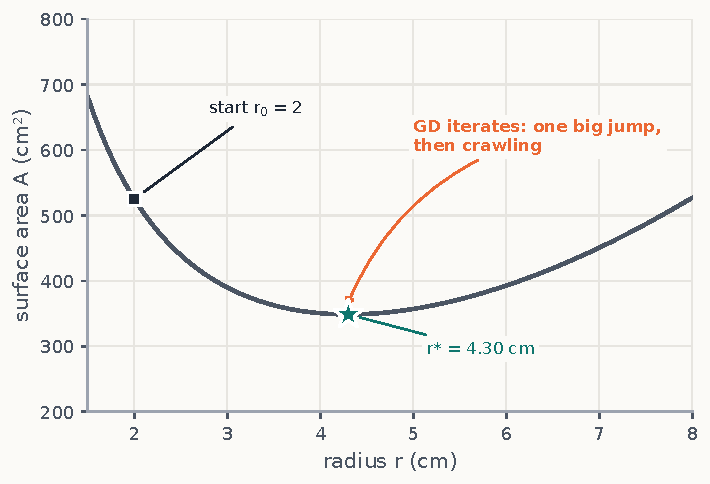
\includegraphics[width=\linewidth, height=0.62\textheight, keepaspectratio]{fig_can_design}
    \end{column}
  \end{columns}
\end{frame}

\begin{frame}{\soltitle{A4}{2}{3}}
  \textbf{(b) GD from $r_0 = 2$, $\alpha = 0.01$.} At $r = 2$ the slope is $A'(2) = 25.13 - 250 = -224.87$, so
  \[
    r_1 = 2 - 0.01(-224.87) = 4.2487 .
  \]
  \begin{center}\small
  \begin{tabular}{@{}c c c c c@{}}
    \toprule
    step & 1 & 2 & 3 & 32 \\
    \midrule
    $r_k$ (cm) & $4.2487$ & $4.2688$ & $4.2811$ & $\ans{4.3013}$ \\
    $A(r_k)$ (cm$^2$) & $348.787$ & $348.754$ & $348.742$ & $348.734$ \\
    \bottomrule
  \end{tabular}
  \end{center}
  The first step is large because the slope is steep where the can is thin. GD then converges, and $|A'| < 10^{-6}$
  after \alert{32} steps.
\end{frame}

\begin{frame}{\soltitle{A4}{3}{3}}
  \textbf{(c) Stability.} Near $r^\star$ the error factor is $1 - \alpha A''(r^\star)$, with $A''(r^\star) = 37.70$:
  \[
    0 < \alpha < \frac{2}{37.70} = \ans{0.0531}
  \]
  With $\alpha = 0.06$ the factor is $1 - 0.06(37.70) = -1.26$, and $|{-1.26}| > 1$:
  \[
    4 \to 4.734 \to 3.842 \to 5.010 \to 3.623 \to 5.463 \to \cdots
  \]
  The radius oscillates between narrow and wide cans, with $A$ \emph{rising} each time. It ends up flipping between
  $r \approx 2.9$ and $7.8$ forever without reaching $r^\star$.
  \begin{warnbox}[Take-away]
    A rate $13\%$ above the limit fails here. Check $\alpha < 2/f''$ before trusting a run.
  \end{warnbox}
\end{frame}

% =====================================================================
%  A5 -- Education: predicting pass or fail (logistic regression)
% =====================================================================
\subsection{A5: Education, pass or fail}
\setprob{A5}

\begin{frame}{\probtitle{A5}{Education: will this student pass?}}
  \begin{probbox}[Problem A5 \hfill Application \quad $\star\star\star$]
    Five students: hours studied $x = (1, 2, 3, 4, 5)$, result $y = (0, 0, 1, 0, 1)$ (1 means pass).
    Model $p = \sigma(wx + b) = 1/(1 + e^{-(wx + b)})$ with the mean cross-entropy loss
    \[
      L(w, b) = -\tfrac1m\textstyle\sum_i\bigl[y_i\ln p_i + (1 - y_i)\ln(1 - p_i)\bigr].
    \]
    \begin{enumerate}[(a)]
      \item The gradients are $\partial L/\partial w = \tfrac1m\sum(p_i - y_i)x_i$ and $\partial L/\partial b = \tfrac1m\sum(p_i - y_i)$.
            Take two GD steps from $(0, 0)$ with $\alpha = 0.5$.
      \item Why can't we just solve $\nabla L = \mathbf 0$ by hand?
      \item Run GD to convergence. Predict the chance of passing after $3.5$ hours, and find the pass/fail boundary.
    \end{enumerate}
  \end{probbox}
\end{frame}

\begin{frame}{\soltitle{A5}{1}{3}}
  \textbf{(a) Step 1 from $(w, b) = (0, 0)$.} Every $p_i = \sigma(0) = 0.5$, and $L = \ln 2 = 0.6931$.
  \[
    p_i - y_i = (0.5,\ 0.5,\ -0.5,\ 0.5,\ -0.5)
  \]
  \[
    \frac{\partial L}{\partial w} = \tfrac15(0.5 + 1 - 1.5 + 2 - 2.5) = -0.1,\qquad
    \frac{\partial L}{\partial b} = \tfrac15(0.5) = 0.1
  \]
  \[
    (w, b)_1 = (0 + 0.05,\ 0 - 0.05) = \ans{(0.05,\ -0.05)}
  \]
  \textbf{Step 2.} Now $p = (0.500,\ 0.512,\ 0.525,\ 0.537,\ 0.550)$ and $L = 0.6850$, lower than before.
  The gradient is $(-0.00024,\ 0.1249)$, so
  \[
    (w, b)_2 = \ans{(0.05012,\ -0.11247)}
  \]
\end{frame}

\begin{frame}{\soltitle{A5}{2}{3}}
  \textbf{(b) No closed form.} Setting the gradients to zero gives
  \[
    \textstyle\sum_i\bigl(\sigma(wx_i + b) - y_i\bigr) = 0,\qquad \sum_i\bigl(\sigma(wx_i + b) - y_i\bigr)x_i = 0 .
  \]
  Here $w$ and $b$ appear inside exponentials, so the equations cannot be rearranged for them.
  GD handles this case: the loss is smooth, but ``slope $= 0$'' cannot be solved.

  \vspace{4pt}
  The loss is \emph{convex} (its Hessian is positive definite), so there is one minimum, and GD from any start
  reaches it. Unlike M1, the starting point does not matter.
\end{frame}

\begin{frame}{\soltitle{A5}{3}{3}}
  \begin{columns}[T]
    \begin{column}{0.5\textwidth}
      \small
      \textbf{(c) After 20\,000 steps}, the gradient is essentially zero ($\approx4\times10^{-16}$):
      \[
        \ans{w = 1.0904,\quad b = -3.8940}
      \]
      with $L = 0.4844$. After $3.5$ hours:
      \[
        p = \sigma(1.0904\times3.5 - 3.8940) = \ans{0.481}
      \]
      The boundary is where $p = 0.5$, i.e.\ $wx + b = 0$:
      \[
        x = -b/w = \ans{3.57\text{ hours}}
      \]
      Above about $3\tfrac12$ hours, the model predicts a pass.
    \end{column}
    \begin{column}{0.48\textwidth}
      \centering
      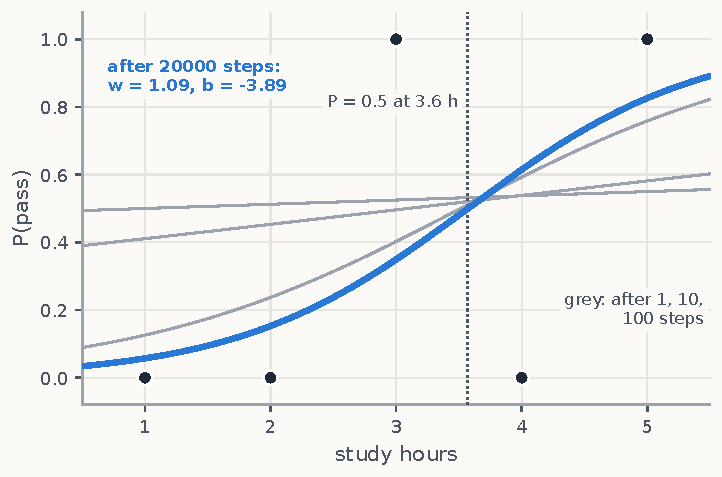
\includegraphics[width=\linewidth, height=0.64\textheight, keepaspectratio]{fig_logistic}
    \end{column}
  \end{columns}
\end{frame}


% ---------------- References -----------------------------------------
\setprob{}
\nextsectionlabel{R}
\nextsectionstop{0}
\section{References}
\begin{frame}[allowframebreaks]{References}
  \scriptsize
  \nocite{*}
  \bibliographystyle{plain}
  \bibliography{bibliography/references}
\end{frame}

\end{document}
